% This is the Reed College LaTeX thesis template. Most of the work
% for the document class was done by Sam Noble (SN), as well as this
% template. Later comments etc. by Ben Salzberg (BTS). Additional
% restructuring and APA support by Jess Youngberg (JY).
% Your comments and suggestions are more than welcome; please email
% them to cus@reed.edu
%
% See http://web.reed.edu/cis/help/latex.html for help. There are a
% great bunch of help pages there, with notes on
% getting started, bibtex, etc. Go there and read it if you're not
% already familiar with LaTeX.
%
% Any line that starts with a percent symbol is a comment.
% They won't show up in the document, and are useful for notes
% to yourself and explaining commands.
% Commenting also removes a line from the document;
% very handy for troubleshooting problems. -BTS

% As far as I know, this follows the requirements laid out in
% the 2002-2003 Senior Handbook. Ask a librarian to check the
% document before binding. -SN

%%
%% Preamble
%%
% \documentclass{<something>} must begin each LaTeX document
\documentclass[12pt,twoside]{reedthesis}
% Packages are extensions to the basic LaTeX functions. Whatever you
% want to typeset, there is probably a package out there for it.
% Chemistry (chemtex), screenplays, you name it.
% Check out CTAN to see: http://www.ctan.org/
%%
\usepackage{graphicx,latexsym}
\usepackage{amssymb,amsthm,amsmath}
\usepackage{longtable,booktabs,setspace}
\usepackage{chemarr} %% Useful for one reaction arrow, useless if you're not a chem major
\usepackage[hyphens]{url}
\usepackage{rotating}
\usepackage{natbib}
\usepackage{todonotes}
\usepackage{hyperref}
\usepackage{verbatim}
\usepackage{epigraph}
\usepackage{lmodern}
\usepackage{caption}
\usepackage{listings}
\usepackage{scrextend}
\usepackage{subcaption}
\lstset{
basicstyle=\small\ttfamily,
columns=flexible,
breaklines=true
}

%% Added for comments
\usepackage{color}
\newcommand{\anna}[1]{{\color{blue}[AR: #1]}}
\newcommand{\new}[2]{{\color{red}#1 [#2]}}
\theoremstyle{definition}
\newtheorem{definition}{Definition}[section]

\setlength\epigraphwidth{8cm}
\setlength\epigraphrule{0pt}
\setlength{\epigraphwidth}{.8\textwidth}

\usepackage{etoolbox}

\makeatletter
\patchcmd{\epigraph}{\@epitext{#1}}{\itshape\@epitext{#1}}{}{}
\makeatother

%% Preface quote stuff
\newlength\longest

%% Graphics path
\graphicspath{ {figures/} }

% Comment out the natbib line above and uncomment the following two lines to use the new
% biblatex-chicago style, for Chicago A. Also make some changes at the end where the
% bibliography is included.
%\usepackage{biblatex-chicago}
%\bibliography{thesis}

\newcommand{\argmax}{\arg\!\max}

% \usepackage{times} % other fonts are available like times, bookman, charter, palatino

\title{Modeling Cell Signaling Networks with Prize-Collecting Subhypernetworks}
\author{Barney Isaksen Potter}
% The month and year that you submit your FINAL draft TO THE LIBRARY (May or December)
\date{May 2016}


%\division{Mathematics and Natural Sciences}
\advisor{Anna M. Ritz}
%If you have two advisors for some reason, you can use the following
\altadvisor{James D. Fix}
%%% Remember to use the correct department!
\department{Interdisciplinary Committee for Mathematics and Biology}
% if you're writing a thesis in an interdisciplinary major,
% uncomment the line below and change the text as appropriate.
% check the Senior Handbook if unsure.
\thedivisionof{The Interdisciplinary Committee for Mathematics and Biology}
% if you want the approval page to say "Approved for the Committee",
% uncomment the next line
\approvedforthe{Committee}

\setlength{\parskip}{0pt}
%%
%% End Preamble
%%
%% The fun begins:
\begin{document}

  \maketitle
  \frontmatter % this stuff will be roman-numbered
  \pagestyle{empty} % this removes page numbers from the frontmatter

% Acknowledgements (Acceptable American spelling) are optional
% So are Acknowledgments (proper English spelling)
    \chapter*{Acknowledgments}
	I would, first and foremost, like to thank my parents, David Potter and Lisa Isaksen. For my whole life they have provided me with immeasurable support, motivated me to always be better, and, of course, fed me. Thank you, Mom  for teaching me to be critical of the world and to be ready to deal with it appropriately. Also, thank you for the enormous amount of medical advice that you are always willing to provide at the drop of a hat. Dad, thank you for giving me a love of education and teaching me all the doors that education can open. Thanks as well for the excellent birding trips that we've taken while I have been at Reed, they were a delight, and I can't wait for more. I would also like to thank my brother, Samuel Jostein Isaksen Potter, for being an excellent source of motivation, entertainment, and poetry (See Preface). Sam, you are an excellent brother, and I can't wait to see what you end up doing with your education.\par
  I'd like to thank a few more members of my family, starting with my grandfather, Odd Isaksen. Thank you, Far Far, for teaching me the importance of mastering a skill and taking care of myself. Thank you, Will, for the excellent adventures, I doubt I'll forget them any time soon. Thank you as well to Rich, Stu, Aunt Ellen, and Uncle Ed for giving me a place where I could escape the stress of Reed whenever I needed it. Finally, I would like to thank my paternal grandparents, Helen and Melvin Potter, for giving me a constant stream of love and support throughout my childhood and teaching me the value of hard work. I miss you both. \par
  Through my time at Reed, I've had the privilege of being supported by some excellent friends, both here and elsewhere. I want to give a huge shout-out to Mari Shiratori Cobb for giving me an astronomical amount of support for the last 2.5 years. I honestly could not have done everything without you. Michael Weiss, thank you for being an amazing friend for the entirety of our tenure at Reed, it has been a pleasure. Caleb Kalisher, thank you for being an excellent friend and duo-queue partner for the last few years. I'd like to give a big thank you to Gordon and Katie for teaching me what it means to be a Reedie, and for giving me a window into what life can be like beyond Reed. Also, thank you very much for all the food both at Jam, and beyond. I would also like to thank my three great friends from beyond Reed: Hailey Boren, Colten Burke, and Trenton Green. Thank you all for being constantly supportive and for being great friends through all the years.\par
  At this point, I would like to thank all the people who have made my Reed education and this thesis possible. First, thank you to my advisors Anna Ritz and Jim Fix. I appreciate all the time and effort that you both have put in to making sure that my education was complete and that my thesis actually worked. I would also like to thank Sarah Schaack, Jeremy Coate, Leigh Latta, and the entire Schaack lab for giving me the opportunity to conduct independent research and learn how much I enjoy bioinformatics. Thank you to Nicole, Heather, and the entire Ritz group for being a great support network during the writing of this thesis. Thank you to my benefactors, your wonderful donations made attending Reed possible for me.\par
  I would like to thank my corporate sponsors for helping me survive and thrive during my time at Reed. I'd like to give a huge thank you to Riot Games, for providing me with one of the best stress relief tools immaginable. Thank you as well to Valve for both giving me an outlet to have some fun during my free time, and provind a platform through which I could learn how interesting and challenging game development can be. Thank you to the Paradox caf\'{e} for giving me the caffeine that I needed to make this thesis possible. Thank you to Gigantic Brewing Company for making the best beer in Portland right next door to Reed. Thank you to Maru, Tea Chai T\'{e}, Tom Yum, the Lutz, and Pambiche for providing great food, drink, and fun that has helped me really enjoy my time in Portland.\par
  Finally, I would like to thank Alan Turing and Ada Lovelace for putting up with so much adversity to make these wonderful machines that we use for work and pleasure possible.\par

% The preface is optional
% To remove it, comment it out or delete it.
    \chapter*{Preface}
	%\epigraph{We can only see a short distance ahead, but we can see plenty there that needs to be done.}{\textit{Alan Turing}}
  \begin{center}
\epigraph{
   It is an unkempt Researcher, \\
  And he stoppeth one of three. \\
  `By thy patched red beard and bloodshot eye, \\
  Now wherefore stopp'st thou me?'
  \bigbreak
  He holds him with his withered hand, \\
  `There was a shrub,' quoth he. \\
  `Hold off! unhand me, red-beard loon!' \\
  Eftsoons his hand dropt he...
  \bigbreak
  He holds him with his bloodshot eye--\\
  The Renn Fayre-Guest stood still, \\
  And listens like a three years' child: \\
  The Researcher hath his will.}{--- \textup{Samuel Jostein Isaksen Potter}}%
\end{center}

    \tableofcontents
% if you want a list of tables, optional
    \listoftables
% if you want a list of figures, also optional
    \listoffigures

% The abstract is not required if you're writing a creative thesis (but aren't they all?)
% If your abstract is longer than a page, there may be a formatting issue.
    \chapter*{Abstract}
	Cell signaling pathways are important tools used by biologists to model how signals are transduced through cells. Though signaling pathways can be (and often are) modeled using graphs, we instead use a generalization known as ``hypergraphs." Using these, we draw from the literature on hypergraphs and their traversal to develop the notion of a ``hypershrub," a multi-source, multi-target generalization of a hyperpath. Drawing from the literature on Prize-Collecting Steiner trees and their applications to biological systems, we create a formulation that finds specific, prize-dense hypershrubs that may be representative of biological phenomena that went previously unnoticed in standard graph representations of the same signaling pathways. Finally, we apply this formulation to the human Hedgehog signaling pathway, and dysregulations therein, related to Basal Cell carcinoma to analyze the effectiveness of our algorithm in real data.

	\chapter*{Dedication}
	I would like to dedicate this thesis to my grandmother, Carol Jane Isaksen, who passed away during the writing of this thesis. Having the opportunity to have you in my family's home throughout high school and college was one of the greatest pleasures that I have had in my life. You were always a kind, loving, and funny grandmother for as long as I can remember. I'll never forget the smiles you had for me and the conversation that we would share every day when I walked through the front door of my family's home. Thank you, grandma, for showing me unconditional love and being one of the most supportive and kind people that I've had the pleasure of meeting. I love you, and I miss you.
    %\item{Born November 15, 1931. dad worked in mines in Wisconsin- Polish immigrant family, mom Norwegian-American. Parents: Leo and Merle Herman. Ended up in pengilly (NE Minnesota by Swan Lake) log house on the lake. Leeches in water. 2 Sisters & a brother, all shared a mattress. Alice, Grandma, Bonnie, Clarence (uncle Punky). Moved to Seattle when she was 6 (gearing up for WWII) to work (grandpa) in the shipyards. Ended up in Bothell. Very close with her dad. Kind of a tom-boy. Didn't really like women. Felt like an outsider in her family. Very funny. Would pick berries in the B-ham summer and lived in the slave quarters. Lived on Norway Hill in Bothell. Met Far Far at a dance in Kenmore. Married Far Far right after that (like 6 weeks). Stay at home mom until mom was in k-garden. Started doing custodial and laundry for the school district. Retired in 1994. She painted. She always wanted to play the drums as a kid in school, but her mom wouldn't let her. She liked Pink Floyd and the Alan Parsons Project. She was a great mother, even though mom was an unappreciative shithead. Would decorate elaborately for Halloween. She really liked animals. Wouldn't wear makeup except lipstick, wouldn't go anywhere without putting on her lips. Sen sens. Bowling league.}

  \mainmatter % here the regular arabic numbering starts
  \pagestyle{fancyplain} % turns page numbering back on

%The \introduction command is provided as a convenience.
%if you want special chapter formatting, you'll probably want to avoid using it altogether

    \chapter*{Introduction}
         \addcontentsline{toc}{chapter}{Introduction}
	\chaptermark{Introduction}
	\markboth{Introduction}{Introduction}
	% The three lines above are to make sure that the headers are right, that the intro gets included in the table of contents, and that it doesn't get numbered 1 so that chapter one is 1.

% Double spacing: if you want to double space, or one and a half
% space, uncomment one of the following lines. You can go back to
% single spacing with the \singlespacing command.
\onehalfspacing
% \doublespacing

Since the discovery of cells by Robert Hooke in 1665, biologists have worked tirelessly to unlock the mysteries of cell function, and over the last half-century, our knowledge of these functions has grown tremendously. An important and growing part of the field of biology has been the increased use of computational methods in helping researchers test pre-existing hypotheses and generate novel hypotheses. Computer-based methodology has been used allowing for a wide range of applications, from DNA and RNA sequence analysis (\cite{humanGenome}) to high-throughput modeling of population growth (\cite{Anderson2005}), to the growing fields concerned with artificial neural networks (\cite{Chon1996}). Notably, in recent years, biologists\footnote{And other scientists, for that matter.} have begun to employ some of the computational tools that computer scientists have been developing for decades. This recent synthesis of fields (see Figure \ref{fig:bioinf_venn}) has created a new area of research, where existing algorithms and computational methodologies are being adapted and honed to help elucidate new meaning from biological data.\par

 \begin{figure}[!h]
   \begin{center}
     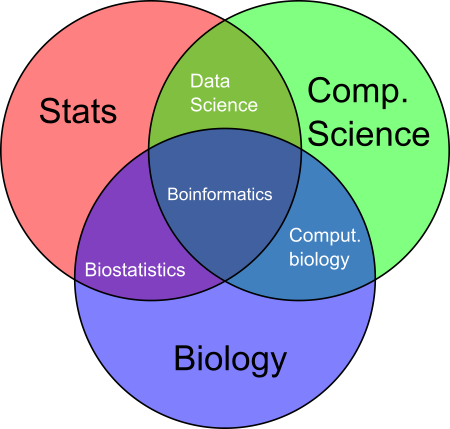
\includegraphics[width=\textwidth/2]{bioinformatics_venn}
   \caption[Fields of bioinformatics.]{A venn diagram of the intersection between the fields of biology, computer science, and statistics. This thesis is primarily concerned with the field of computational biology. Image from \url{https://genomejigsaw.wordpress.com/2015/09/27/faq/}, Marek Cmero.}
   \label{fig:bioinf_venn}
   \end{center}
 \end{figure}

 \section{Signaling Pathways}

 One of the most promising areas where computational methods are now being applied concerns the study of signaling pathways within cells. Generally, signaling pathways represent what we currently know about how proteins and small molecules interact within cells in order to propagate signals throughout the cell, ultimately changing the behavior of the cell. We find cell signaling pathways remarkable because understanding how signaling information spreads throughout a cell helps us to better grasp dysregulations which result in changes to cellular dynamics. These dysregulations often manifested in heterogeneous diseases such as cancer\footnote{As well as many other diseases in which signaling pathway dysregulations have been implicated.} (\cite{Taylor2009}). Signaling pathways have been studied for years, and they have often been represented visually as flow diagrams (Figure \ref{fig:shh}) Recently, however, researchers have begun to ``convert" the traditionally-drawn diagrams of signaling pathways into mathematically-interesting structures, for which known algorithms can be employed to learn more about the signaling pathways.\par

 \begin{figure}[!h]
   \begin{center}
     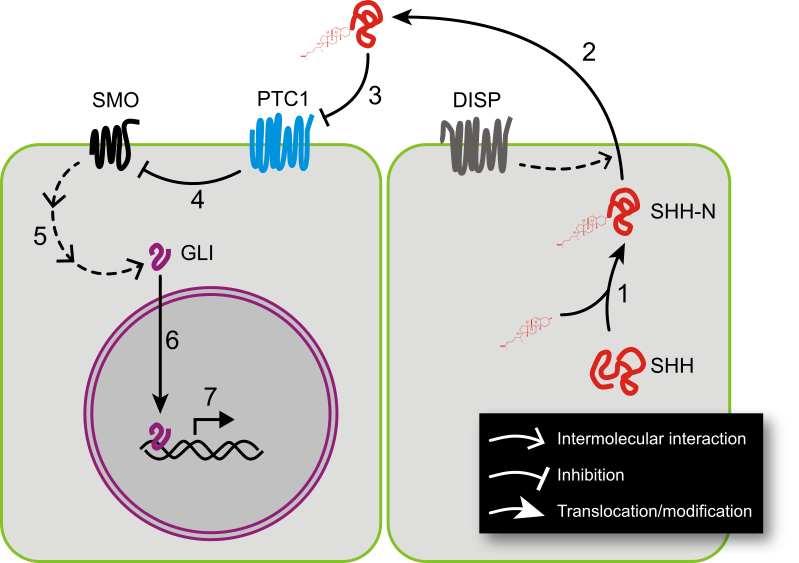
\includegraphics[width=4in]{Sonic_hedgehog_pathway}
   \caption[Sonic hedgehog signal transduction.]{A traditional representation of the Sonic Hedgehog signaling pathway. By Fred the Oysteri. The source code of this SVG is valid. This vector graphics image was created with Adobe Illustrator., GFDL, \url{https://commons.wikimedia.org/w/index.php?curid=36313869}}
   \label{fig:shh}
   \end{center}
 \end{figure}

 \section{Network Representations}

  To build a mathematical model of cell signaling pathways, we often use a graph as an abstract representation of the structure of the pathways. Graphs were first described by Euler in 1736 (\cite{Shields2012}) to help explain the complex relationships between objects\footnote{In Euler's case, the seven bridges of K\"{o}nigsberg.} in a concise, well defined way. For the purpose of this thesis, the word ``graph\footnote{A term coined by James Joseph Sylvester in 1878 (\cite{Biggs1986}).}" will refer to this model of real-world pehnomena. A graph, $G=(V,E)$ is a structure that represents a set of objects, $V$ referred to as \textit{nodes} or \textit{vertices} and pairwise connections between them, $E$ referred to as \textit{edges}. Edges in a graph can either be \textit{undirected} or \textit{directed} (shown in Figure \ref{fig:simple_graph_du}), meaning that they go from one node (the \textit{tail}) to another node (the \textit{head}). We define a \textit{subgraph}, $G^\prime$, of $G$ as the graph $G^\prime=(V^\prime,E^\prime)$ where $V^\prime \subseteq V$, $E^\prime \subseteq E$. Furthermore, we define an \textit{induced vertices} as the subgraph that arises from a subset of edges, $V(E^\prime)$.\par

  One of the greatest advantages of using graphs as modeling tools is the wealth of graph algorithms that have been developed since Euler first proposed problems on graphs in 1736. These algorithms make it simple for graphs that are representative of real biological data to be queried for interesting substructures (i.e. shortest path between two nodes, modularity of a graph, or subgraphs that satisfy certain parameters) which can themselves be analyzed to determine whether they represent a biologically meaningful phenomena.\par

  \begin{figure}[!h]
    \begin{center}
      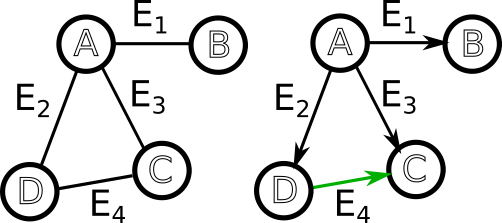
\includegraphics[width=\textwidth/2]{simple_graph_du}
    \caption[Undirected \& Directed Graphs]{A simple undirected graph (left) and its directed counterpart (right). The highlighted edge has node $D$ as its tail and $C$ as its head.}
    \label{fig:simple_graph_du}
    \end{center}
  \end{figure}

  We use graphs to model relationships that we observe in the world, and sometimes it is useful to have more information than just the presence or absence of edges. One way that we can expand the information that our graphs contain is through weighting. When we weight a graph, we generally assign values to the edges (though sometimes the nodes as well) to attach additional information to each edges, other than which nodes they connect. Weights can represent many different conditions, and often help apply real-world meaning to a graph that is being used as a modeling tool. For instance, if one had a graph where the nodes were representative of locations, then the weights of the edges could be used to show the distance between the nodes. One could also use a graph to represent a group of lab-mates who play streetball together during the summer, with weighted edges representing the likelihood that any two people will play on the same team. In the case of this thesis, we will use a combination of edge and node weighting to build subgraphs that may be biologically interesting using gene expression data. Formally, we think of our graph $G=(V,E)$ as a strucure weighted by a function $w:E \rightarrow \mathbb{Q}$ that assigns weights to edges. Similarly, we can assign values to nodes through some function $\ell:V \rightarrow \mathbb{Q}$.\par

   \subsection{Walks, Paths, Connectivity, and Trees}

   In graphs, it is useful to define a way to traverse the graph, through the nodes and edges. We define a \textit{walk} in a graph as an alternating series of nodes and edges, such that each edge included in the walk is adjacent to the two nodes incident upon it. An example of one such walk, $W$ in the undirected graph from Figure \ref{fig:simple_graph_du} is:\par

   \begin{equation*}
     W = A \cdot E_2 \cdot D \cdot E_2 \cdot A \cdot E_1 \cdot B
   \end{equation*}

   Furthermore, we can define a \textit{directed walk} in a directed graph as a walk that respects the direction of the edges in the graph. Additionally, we define a \textit{path} (or a \textit{directed path}, in directed graphs) as a walk for which there are no repeated vertices or edges. We say that a graph is \textit{connected} if, for any pair of nodes in the graph, there exists a path between those two nodes. It is important to note that the endpoints of both paths and walks are always nodes, not edges. For example, in the directed graph shown in Figure \ref{fig:simple_graph_du}, one possible path from $A$ to $C$, is:\par

   \begin{equation*}
     P = A \cdot E_2 \cdot D \cdot E_4 \cdot C
   \end{equation*}

   Using our definition of a path, we can also define a \textit{cycle} as a path for which the start and end nodes are the same. Using this definition, we can also say that any path or graph that does not contain any cycles as an \textit{acyclic} path or graph. Finally, we can define a \textit{tree} as any undirected graph that is connected and acyclic. This means that for any pair of nodes in a tree there exists exactly one path between them.\par

   \subsection{Spanning Trees and Steiner Trees}

   It is often useful to find subgraphs in a given graph that fulfill specific parameters. These subgraphs are often formulated as a decision question: ``Given a graph $G$ and a set of parameters, does subgraph $G^\prime$ of $G$ exist that meets all of the specified parameters?" An example of one such graph is a complete graph, shown in Figure \ref{fig:complete_graphs}. A complete graph of $m$ nodes (\textit{k}-$m$) is defined as an undirected graph for which each node is connected to each other node by exactly one edge.

   \begin{figure}[!h]
     \begin{center}
       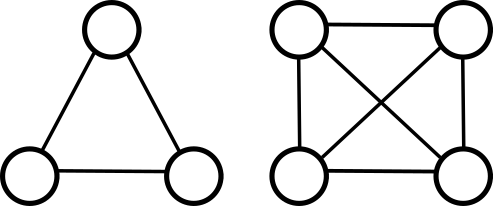
\includegraphics[width=\textwidth/2]{complete_graphs}
     \caption[Complete Graphs \textit{k}-3 and \textit{k}-4.]{Complete graphs with three and four nodes.}
     \label{fig:complete_graphs}
     \end{center}
   \end{figure}

   We could then, for example, ask whether a graph on $n$ nodes had a complete subgraph of size $m$. Figure \ref{fig:complete_graphs} (left), for example, contains a complete subgraph of size 3, but not one of size 4. These complete subgraphs are called ``cliques", where a clique of a certain size is an $m$-clique. We formulate this decision question as:\par

   \bigbreak

   \hfill\begin{minipage}{\dimexpr\textwidth-2cm}
   \paragraph{Given.}An undirected graph $G=(V,E)$ and some integer $m$.
   \paragraph{Find.}Subgraph $G^\prime = (V^\prime,E^\prime)$ subject to:
   \begin{itemize}
     \item{$E^\prime = \{(u,v) \,|\, u,v \in V^\prime\}$}
     \item{$|V^\prime| = m$}
   \end{itemize}
\xdef\tpd{\the\prevdepth}
\end{minipage}


   \subsubsection{Spanning Trees.}
   One structure that we can look for in a graph is a \textit{spanning tree}, a tree that reaches every node in the graph while still conforming to all the constraints that define a tree. The spanning tree decision question is formulated as:

   \bigbreak

   \hfill\begin{minipage}{\dimexpr\textwidth-2cm}
   \paragraph{Given.}An undirected graph $G=(V,E)$.
   \paragraph{Find.}$R \subseteq E$ subject to:
   \begin{itemize}
     \item{$R$ contains no cycles}
     \item{$R$ connects $V$}
     \item{$V(R) = V$}
   \end{itemize}
\xdef\tpd{\the\prevdepth}
\end{minipage}



   \subsubsection{Steiner Trees.}
   While spanning trees are useful substructures, sometimes we want to find a subtree that only includes certain nodes in the graph, but maybe not others. If this is the case, we can construct a slightly altered version of a spanning tree called a \textit{Steiner tree}\footnote{Named after Swiss mathematician Jakob Steiner.} We formulate this decision problem:

   \bigbreak

   \hfill\begin{minipage}{\dimexpr\textwidth-2cm}
   \paragraph{Given.}An undirected graph $G=(V,E)$ and some $T \subseteq V$.
   \paragraph{Find.}$S \subseteq E$ subject to:
   \begin{itemize}
     \item{$S$ contains no cycles}
     \item{$S$ connects $T$}
   \end{itemize}
\xdef\tpd{\the\prevdepth}
\end{minipage}

   \bigbreak

   Furthermore, we call any node that is included in the Steiner tree, but that is not a member of $T$ a Steiner node. Figure \ref{fig:graph1} gives an example of both spanning and Steiner trees.

   \begin{figure}[!h]
     \begin{center}
       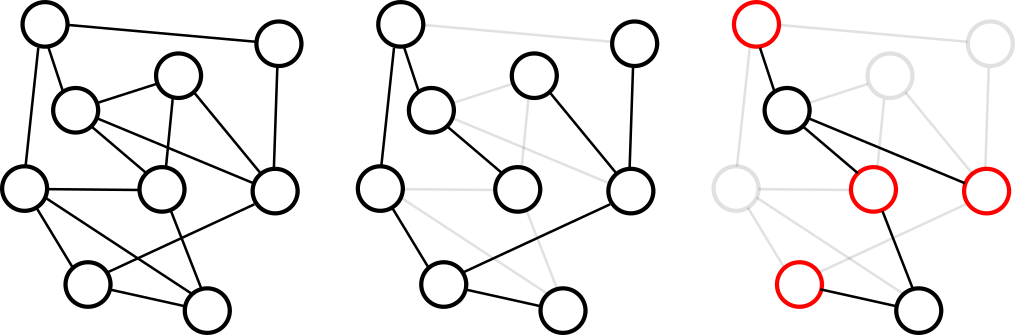
\includegraphics[width=\textwidth]{graph1}
     \caption[Spanning and Steiner trees.]{A graph \textit{(left)} along with a spanning tree \textit{(center)} and a Steiner tree \textit{(right)} within. In the Steiner tree, the red nodes are target nodes and the black nodes are the Steiner nodes.}
     \label{fig:graph1}
     \end{center}
   \end{figure}

 \section{Optimization}
 While decision questions are useful for querying graphs, we often seek solutions that fulfill some notion of ``optimal". In these cases, instead of formulating a decision problem, we instead formulate an optimization problem. Generally, optimization problems require us to use weighted graphs, rather than unweighted, so that some objective function can be optimized. For example, we can find a minimum weight spanning tree by solving the optimization problem:

 \bigbreak

 \hfill\begin{minipage}{\dimexpr\textwidth-2cm}
 \paragraph{Given.}An undirected graph $G=(V,E)$ and some weight function $w:E \rightarrow \mathbb{Q}^+$.
 \paragraph{Find.}$R \subseteq E$ that maximizes:
 \begin{align*}
  o(R)=\sum_{e \in E}w(e)
 \end{align*}
 subject to:
 \begin{itemize}
   \item{$R$ contains no cycles}
   \item{$R$ connects $V$}
   \item{$V(R) = V$}
 \end{itemize}
\xdef\tpd{\the\prevdepth}
\end{minipage}

Similarly, we can define a minimum weight Steiner tree:

 \bigbreak

 \hfill\begin{minipage}{\dimexpr\textwidth-2cm}
 \paragraph{Given.}An undirected graph $G=(V,E)$ and some weight function $w:E \rightarrow \mathbb{Q}^+$.
 \paragraph{Find.}$S \subseteq E$ that maximizes:
 \begin{align*}
  o(S)=\sum_{e \in E}w(e)
 \end{align*}
 subject to:
 \begin{itemize}
   \item{$S$ contains no cycles}
   \item{$S$ connects $T$}
 \end{itemize}
\xdef\tpd{\the\prevdepth}
\end{minipage}


  \subsection{Prize Collecting Steiner Trees}
  It is often the case that there are multiple possible Steiner trees, and we may want to find one (or more) that fulfills some notion of optimality. Most often, we want to find the Steiner tree from a set of candidate Steiner trees that will be minimal. In the case where the parent graph is unweighted, this will mean that the minimal Steiner tree is the one that contains the fewest number of edges. Similarly, in a weighted graph, we say that the minimum weight Steiner tree is the for which the sum of its edge weights is smaller than the sum of the edge weights of all other candidate Steiner trees.\par

  \begin{figure}[!h]
    \begin{center}
      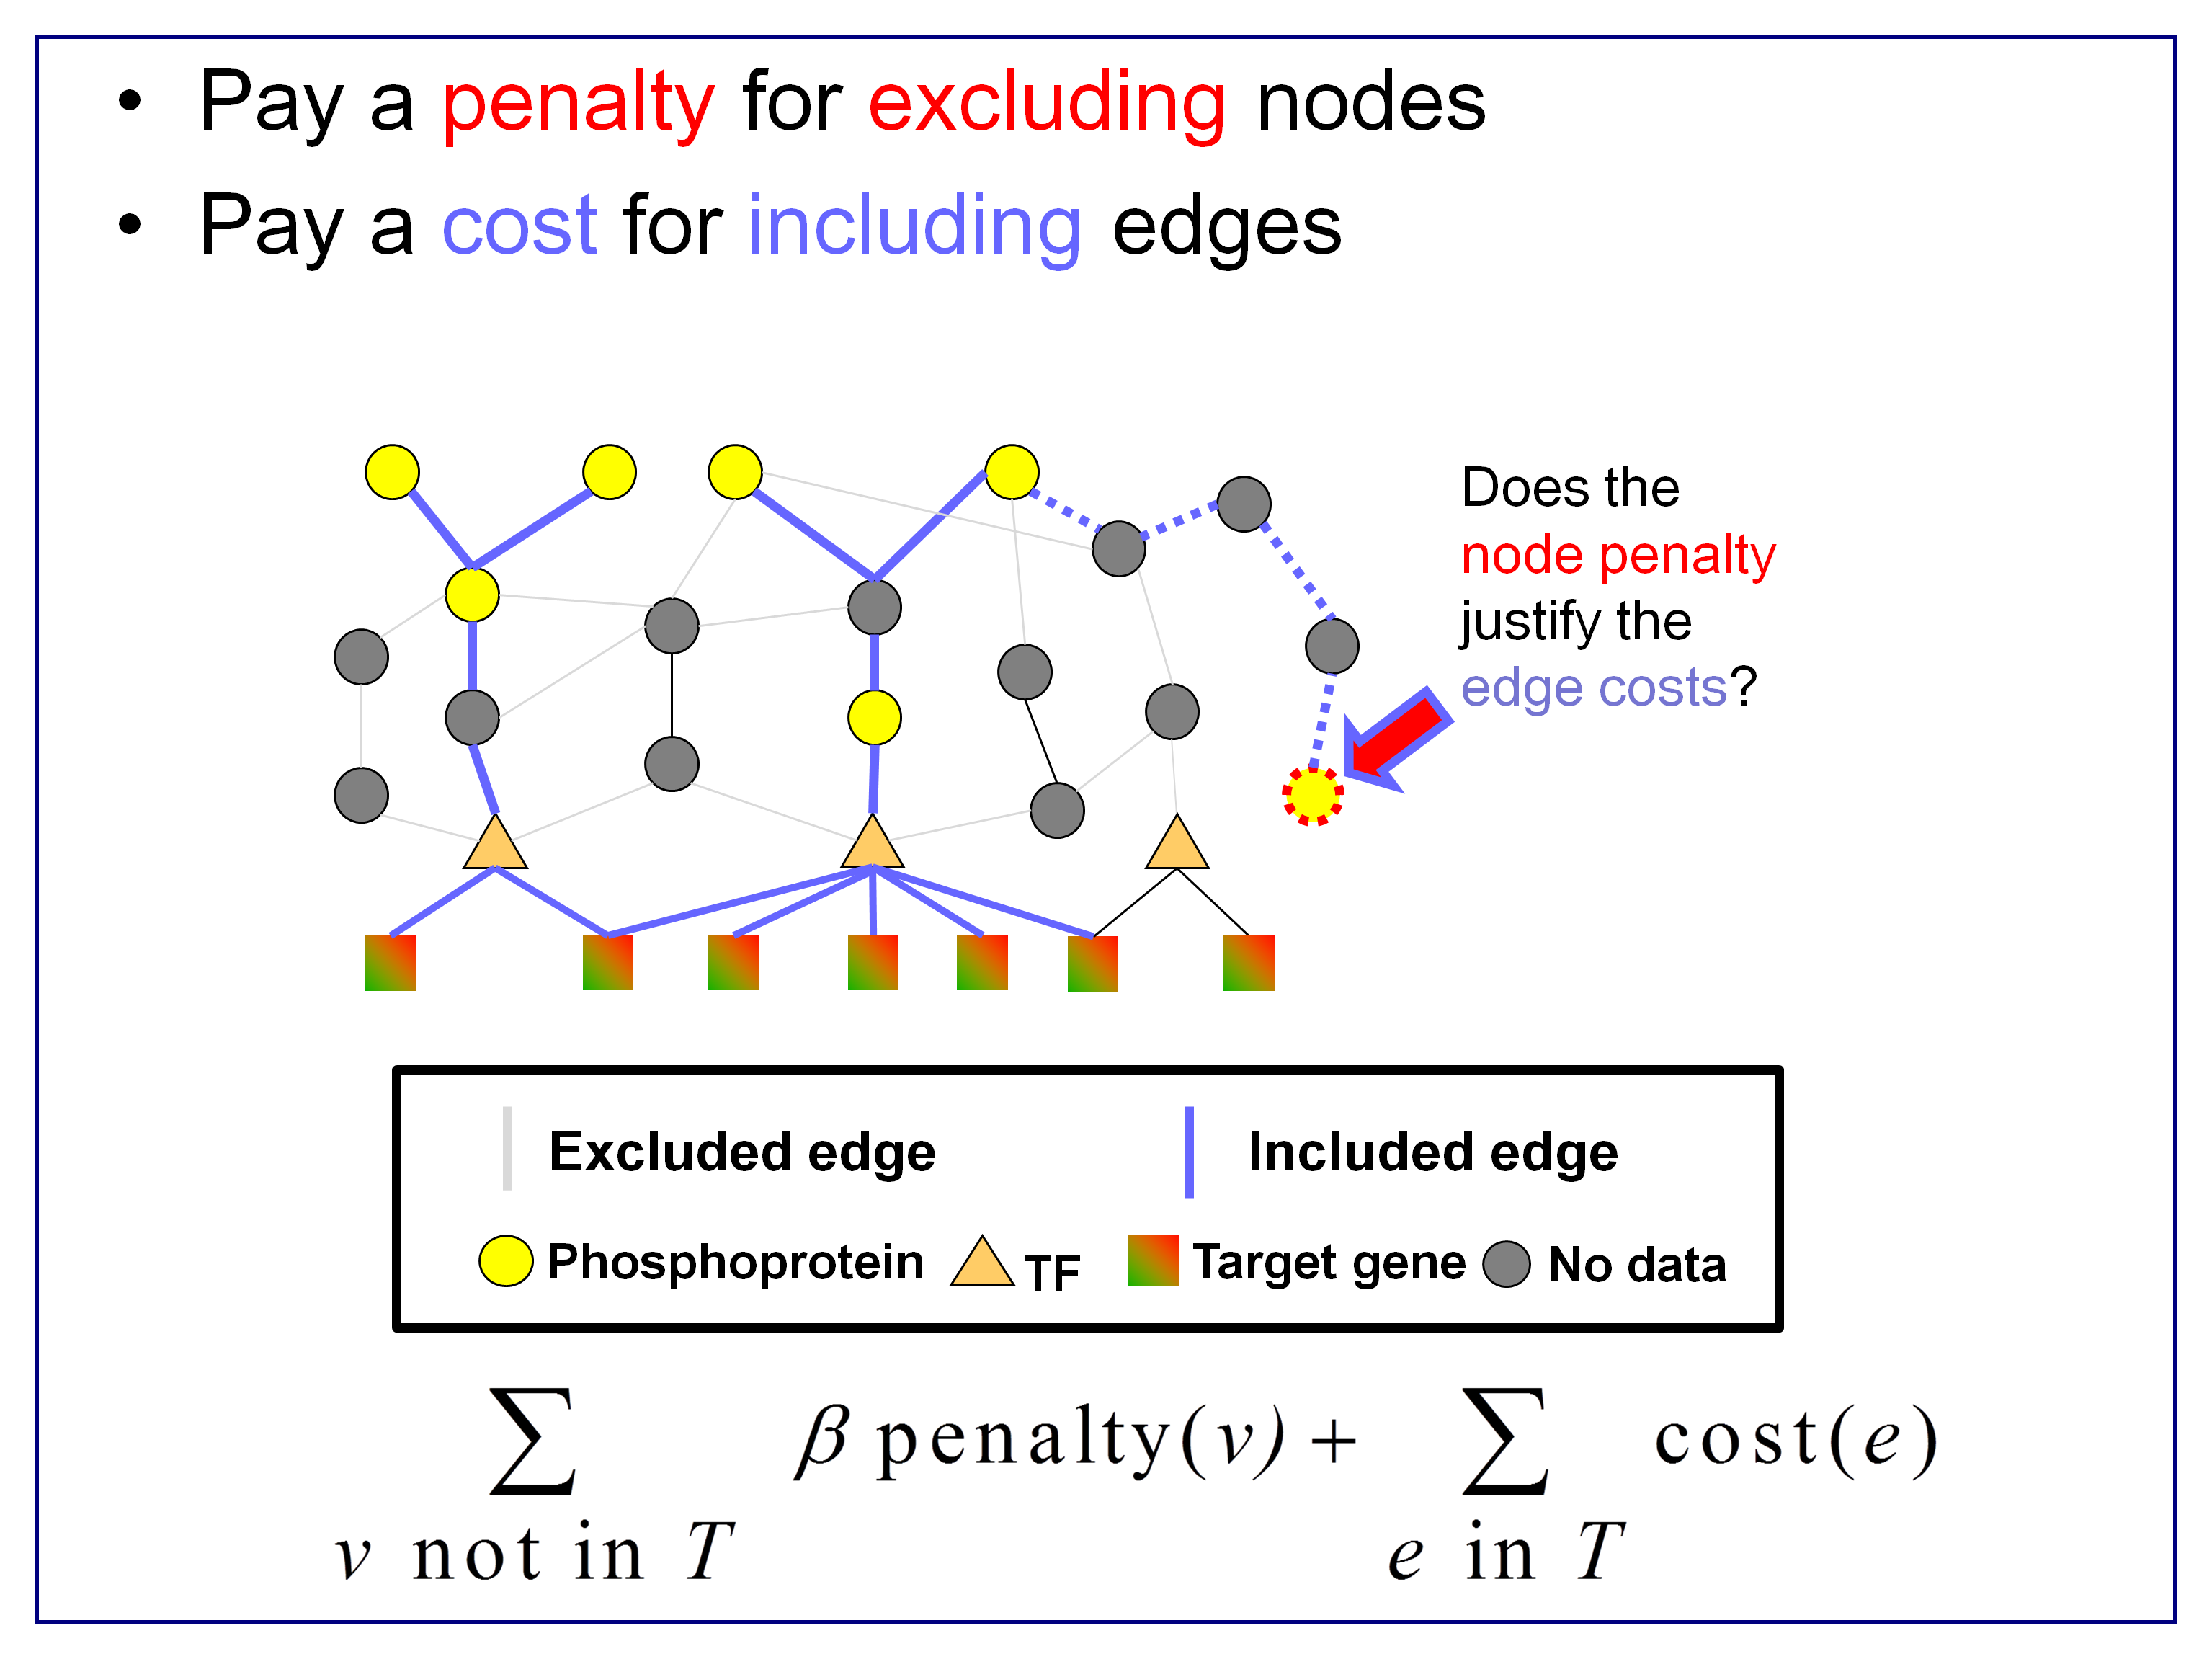
\includegraphics[width=4in]{PCST}
    \caption[Prize-Collecting Steiner Tree]{In protein-protein interaction networks, we want to find the smallest possible subgraph that captures as much prize as possible. One way to find this is by searching for a Prize-Collecting Steiner Tree. Image (c) Copyright by Ernest Fraenkel 2016, reprinted with permission.}
    \label{fig:PCST}
    \end{center}
  \end{figure}

  We often do not just want to find a Steiner tree that explains a fixed target set, but rather want to loosen the constraints to let the exact nodes that are included in a subnetwork be determined algorithmically. This is particularly useful when we are examining biological signaling pathways, where we often have continuous data for a large subset of nodes because of high-throughput transcriptomics and proteomics. In this case we can assign values to some of the nodes in a graph based on available data. These so called ``prizes" are used in lieu of a target set, to quantify how valuable a given node is, if it is included in the subnetwork. Using these prizes, and some scheme of edge weighting, we formulate an optimization problem to find subnetworks that hopefully capture highly-prized nodes, while avoiding costly edges (Figure \ref{fig:PCST}). We call this subgraph a \textit{Prize-Collecting Steiner tree}. We can formally define a Prize-Collecting Steiner tree through the optimization problem:\par

  \bigbreak

  \hfill\begin{minipage}{\dimexpr\textwidth-2cm}
  \paragraph{Given.}An undirected graph $G=(V,E)$, node prize function $g:V \rightarrow \mathbb{Q}^+$, and edge cost function $c:E \rightarrow \mathbb{Q}^+$.
  \paragraph{Find.}$S \subseteq E$ that maximizes:
  \begin{align*}
   o(S) = \sum_{v \in V(S)}g(v) - \sum_{e \in S}c(e)
  \end{align*}
  subject to:
  \begin{itemize}
    \item{$S$ contains no cycles}
    \item{$S$ connects $V(S)$}
  \end{itemize}
\xdef\tpd{\the\prevdepth}
\end{minipage}

\subsection{Algorithmic Complexity}
At this point, we should take a moment to address the difficulty of computing solutions to these formulated problems. The decision and optimization questions that we just laid out are all classic problems in the theory of algorithms. The spanning tree and minimal spanning tree problems end up being easy to solve, that is, they can be solved by algorithms that run in polynomial time. We call the class of decision problems that can be solved in polynomial time \textbf{P}. The Steiner tree problem, and its prize-collecting variant, on the other hand, are believed to be much harder to solve algorithmically. There are currently no theorized algorithms that can solve these problems in polynomial time. Instead, these belong to the class of \textbf{NP-complete} problems (\cite{Garey1979}).\par

We will be formulating problems that are generalizations of the Prize-Collecting Steiner tree problem, including ones that are \textbf{NP-complete}. The algorithmic complexity of the problems we formulate will not not be directly addressed in this thesis. We will instead use a type of problem-solving that can give us exact solutions to this class of questions, using solvers that often work well in practice. We formulate our problems as integer linear programs (ILPs)\footnote{Incidentally, ILP problems are also \textbf{NP-complete}.}.

 \section{Integer Linear Programming}

  There are many kinds of algorithms used to find interesting subnetworks in graphs and hypergraphs.  For this thesis, we use a type of programming known as \textit{integer linear programming}. Integer linear programs (ILPs) solve for the optimal solution(s) to an objective expression, subject to a set of linear constraints (\cite{Papadimitriou1998}). In our case, the set of variables, $\mathbf{x}$, are all binary variables, which will represent whether a given part of the graph is included in the solution. If variable $\mathbf{x}_i$ is equal to 0 in the solution, the part of the graph with which it is associated will not be present in the optimal solution. Similarly, if $\mathbf{x}_i$ is equal to 1, its associated graph component is present in the optimal solution.\par

  The canonical form of an ILP is:\par

  \begin{align}
    \text{Maximize: }\quad&\mathbf{c^Tx}\label{eq:obj_canonical}\\
    \text{Subject to: }\quad&\mathbf{Ax}\leq\mathbf{b}\text{,}\label{eq:constA}\\
    &\mathbf{x} \geq 0 \text{,}\label{eq:constB}\\
    \text{and } \quad & \mathbf{x} \in \mathbb{Z}^n \label{eq:constC}
  \end{align}

  In this form $\mathbf{x}$ is the vector of binary variables for which the program is solving, $\mathbf{c}$ and $\mathbf{b}$ are vectors and $\mathbf{A}$ is a matrix, all of which take integer values. For this thesis IBM ILOG CPLEX Optimization Studio (CPLEX) was used to optimize input ILPs which were input in the form of LP files (\texttt{.lp}, see Appendix A).

 \section{Goals of this Thesis}

 The goal of this thesis is to generate an algorithm that will create subnetworks in a generalization of a graph called a \textit{hypergraph}\footnote{This will be defined both informally and formally later.}. The sub-hypergraph generated by this algorithm should use weights on the edges and nodes of the hypergraph to find a subnetwork that will minimize the total cost of induced edges while maximizing the value of reached nodes. Furthermore, the output should not contain disconnected subgraphs, and it should have some sort of ``flow" going from an undetermined (i.e. not pre-specified) set of nodes, $S$ to another set of nodes, $T$. In addition to formally defining and solving for this target subnetwork, this thesis will find a way to build a network from publically available signaling pathway data, and weight that network in a meaningful way.\par

 Following this, we will discuss the implementation of the algorithm in a weighted hypernetwork that is representative of the Hedgehog signaling pathway in humans. In particular, we will analyze this network after we weight it according to differential gene expression between healthy patients, and ones with Basal Cell carcinoma.

 Ultimately, we will create a software package that anyone could use to build hypergraphs from available data, and to query that hypergraph for potential hypotheses about signaling pathway dysregulations, based on a weighting scheme that the user can apply easily.\par

\chapter{Cell Signaling Networks}

Cell function is governed by countless interactions between proteins, nucleic acids, lipids, carbohydrates, and many other small molecules.  The interactions between all of these components form what we call \textit{protein-protein interaction} (PPI) networks, which are responsible for almost every process within a cell (\cite{Taylor2009}). Furthermore, we often think about specific sub-networks that explain important biological phenomena (hormone secretion, transcriptional regulation of a gene, or response to a particular stimuli are all examples). We refer to these subsets of the larger PPI network as \textit{cell signaling pathways}. We use cell signaling pathways to describe how many of the most basic reactions within cells cause propagations of information, and the results of those signals.  Some of the most important types of interactions that we see in cell signaling networks include the assembly and destruction of protein complexes, how small molecules such as ATP interact with proteins, the cascade of events that can occur after a membrane-bound protein is bound by a ligand, or where negative feedback loops exist that can have an effect on cell function.  Historically, PPI networks have been a useful tool for compiling knowledge about individual interactions that have been studied \textit{in situ}, so that larger-scale patterns of interaction can be examined, and both communicated easily and analyzed algorithmically. In recent years, there has been a push to find ways to accurately model these networks so that they can be used to predict potential areas of future research (\cite{Haverty2004}), in particular, by using graph-based methods (\cite{Aittokallio2006}).\par

There are a multitude of different forms of cell signaling pathways\footnote{As well as intercellular signaling networks and metabolic cell functions that are not triggered externally.}, responsible for many types of cell functions, but we will use the example of a cell changing its gene expression in response to an external stimuli as a general model for signaling pathways. In these cases, there are a few key steps that result in signal transduction throughout the cell. First, a trans-membrane protein will undergo a conformational change in response to a particular ligand\footnote{A small molecule that typically will bind to a trans-membrant, initiating a cascade of events (i.e. the signal that starts the process).}. Typically, this signal will be some sort of messenger molecule to which the cell needs to respond. The change in conformation results in a cascade of interactions between proteins and other small molecules within the cell. Some of the changes that can result from this cascade of signaling are protein complex assembly, complex degradation, conformational changes to other proteins, phosphorylation, or dephosphorylation (among many other reactions). The ultimate result of this signaling cascade is a change in one or more transcription factors, proteins that bind to DNA, and regulate the rate of transcription of DNA to mRNA. The ultimate result of this pathway will be a change in the expression of one or more genes within the cell, and possibly the start of new signaling pathways.\par

\paragraph{Computational Methods.}
Signaling pathways are of particular importance because they are often dysregulated in heterogeneous diseases such as cancer (\cite{Taylor2009}). Because of this, researchers' ability to obtain accurate information about signaling pathways, and their ability to interpret that information may help them to deduce interactions whose dysregulation may be implicated in a particular disease. As our network algorithms grow and become more accurate, we will become increasingly able to develop computational methods to mine these networks for novel hypotheses about the causes of heterogeneous diseases. Additionally, as the databases become more complete, cross-pathway interactions may begin to be documented that would not otherwise be apparent upon studying individual pathways. The development of new computational techniques may help elucidate regulatory changes in areas where different pathways, once modeled as discrete, overlap. If specific areas where there is meaningful overlap between two or more cell singnaling networks could be identified they could lead to new hypotheses that researchers could investigate \textit{in situ}.\par
Furthermore, while past research has found many individual proteins and pathways that are implicated in particular diseases, our ability to observe or quantify certain elements that could be playing an important role in pathway dysregulation is limited by our current sampling methods (RNA-Seq, microarray, etc). The development of more nuanced algorithms could increase our ability to implicate proteins that we cannot currently observe being dysregulated because of how protein expression in cells is currently quantified.\par

Beyond individual signal transduction pathways, it is useful to think of the set of all known interactions together. We refer to this object as an \textit{interactome}, and our ability to analyze it computationally could lead to discovery (or at least postulation) of completely novel signaling networks. By examining the interactome for a species, and weighting it appropriately, it may be the case that we are able to elucidate sets of interactions that had been observed separately, but have not yet been correlated with each other. A simple case of this would be if we find that one signaling pathway was to lead directly into another, that is, the outputs of the first pathway were the inputs to the other. Though interactions between multiple networks as simple as in this example are likely to have already been observed, it could be the case that an algorithm could find that there is some ``chain" of connections between one network and another, or that there was some form of crosstalk between some of the components of two networks. If we could find this type of interaction, it would help researchers understand the extent to which a change in one network may affect another.\par

\begin{figure}[h]
  \begin{center}
    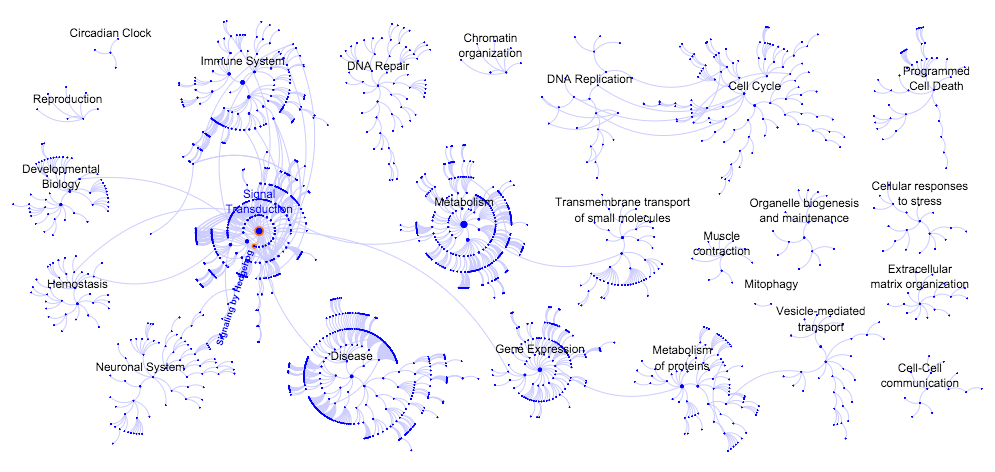
\includegraphics[width=\textwidth]{human_interactome}
  \caption[Human interactome]{The entire human interactome, as displayed by the Reactome interactive pathway browser. Each dot actually represents a discrete signaling pathway.}
  \label{fig:human_interactome}
  \end{center}
\end{figure}

\section{PPI Databases}

In recent years, there has been a push to start curating what is already known about cell signaling, and publishing these networks online (\cite{Bauer-Mehren2009}, \cite{Cusick2009}). Many of these databases have been made available to the public so that the data that they contain can be used collaboratively by anyone. Some of these networks are the Reactome database (\texttt{reactome.org}; \cite{Matthews2009}), NetPath (\texttt{netpath.org}; \cite{Kandasamy2010}), and SPIKE (\path{http://spike.cs.tau.ac.il/spike2/}; \cite{Paz2011}).\par
The purpose of signaling pathway databases is twofold: to create repositories of known interactions so that they can be easily referred to and viewed in a zoomable, searchable manner (\cite{Hu2007}), and so that researchers can take advantage of the computational tools that alerady exist to find novel areas of research from these manually-curated networks (\cite{Karlebach2008}, \cite{Battle2010}). These more modern pathway interaction databases are much smaller than their earlier, non-curated counterpart, but contain much higher confidence interactions making them better candidates for applying computational methods.\par

\section{Signaling by \emph{Hedgehog}: A Case Study}

One example of a cell signaling pathway that has a variety of biological consequences is the \textit{Hedgehog} (Hh) signal transduction network. Hedgehog is a protein that helps regulate limb formation during early development, cell development, differentiation, and the development of neural tubes (\cite{Hui2011}). Hedgehog has been implicated in the development of basal cell carcinoma\footnote{Basal cell carcinoma is one of the most common form of cancer in humans (\cite{Rubin2009}). Basal cell carcinoma is of particular interest to the author of this thesis, as he was diagnosed with and treated for BCC, which motivated the choice of this signaling pathway for analysis in this thesis.} (BCC) when it is overexpressed (\cite{Dahmane1997}). Additionally, it has been shown that Hh has powerful effects on the proper layout and development of tissues in mammals, and it has been proposed that Hh is responsible for assisting with stem cell assisted tissue regeneration in adult mammals (\cite{Ahn2005}).

\begin{figure}[h]
  \begin{center}
    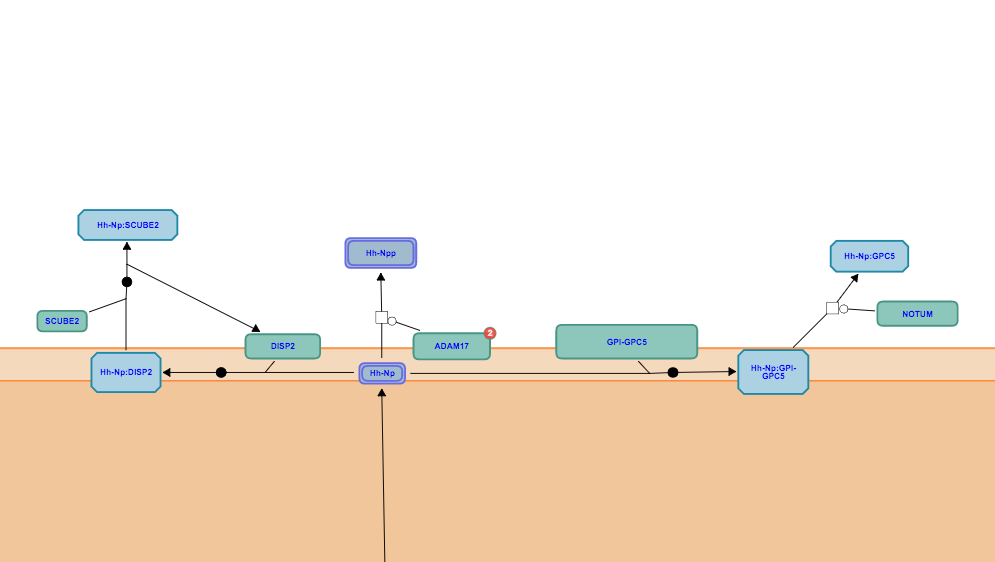
\includegraphics[width=\textwidth]{Hh-Np_secretion}
  \caption[Hedgehog secretion in \textit{Homo sapiens}]{Hh-Np secretion, as shown by \texttt{reactome.org} in \textit{Homo sapiens}.}
  \label{fig:Hh-Np_secretion}
  \end{center}
\end{figure}

The best studied part of the human Hh pathway involves the ligand Sonic Hedgehog (SHH), particularly the behavior of its ~20kDa N-Terminal domain (SSH-N). When SSH-N reaches the Patched-1 (PTCH1) trans-membrance receptor, it causes a conformational change. This causes the release Oxysterol that was previously bound to PTCH1, preventing PTCH1 from inhibiting Smoothened (SMO) (\cite{Carpenter1998}). The relief of inhibition of SMO encourages the acivation of the GLI family of transcription factors. This family includes two activators, Gli1 and Gli2; it also contains one repressor, Gli3 \cite{Rahnama2006}. The end result of the Hh signaling pathway is that the activated transcription factors lead to changes in expression of a large set of Hedgehog target genes.

The Hedgehog signaling pathway makes a useful example for applying computational methods and graph-based modeling, since the network is small enough to look at manually, but also complex enough that its analysis is nontrivial. Furthermore, because it has been implicated with BCC, along with many other forms of cancer, data for weighting signaling networks are available through public databases such as The Cancer Genome Atlas (\texttt{http://cancergenome.nih.gov/}). These factors make it an excellent choice as an example network for testing new hypergraph algorithms.\par

Now that we have an understanding of what signaling pathways and protein interaction networks are, our next step is to develop the appropriate tool with which to model them. To do so, we will now describe a generalization of a graph, known as a hypergraph. We will then describe a new way to query hypergraphs that will find important subnetworks, which we call hypershrubs, that may reveal biologically interesting phenomena that current computational methods fail to capture.\par

\chapter{Hypergraphs \& Hyperpaths}

In order to model cell signaling pathways computationally, it is first necessary to choose the correct computational object to represent our data. For this, we can use graphs, but there are ways in which graphs are not the ideal structure, and leave some things to be desired. In particular, when we are modeling networks such as cell signaling networks that contain a richness of information, reduction to graphs causes some of this information to be lost. Instead of using graphs, we will define a generalization of a directed graph, called a directed hypergraph, and use it to model cell signaling pathways and PPI networks.\par

Our ultimate goal will be to show why directed hypergraphs are a good candidate for representing cell signaling pathways. Then we will seek meaningful subhypernetworks, in the form of a precise hypernetwork structure we call a hypershrub, explored more carefully in the next chapter.

\begin{figure}[h]
  \begin{center}
    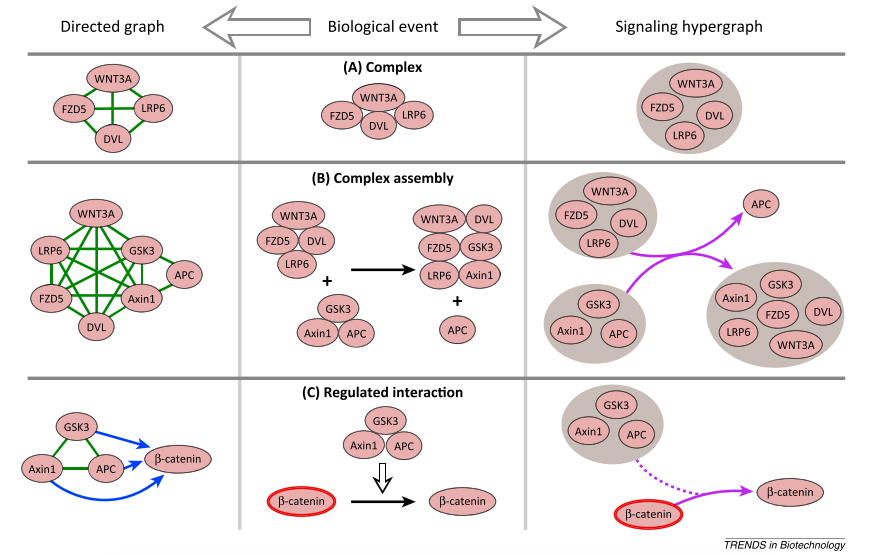
\includegraphics[width=\textwidth]{anna_fig}
  \caption[The issue with standard graphs.]{Standard graphs are not always the best tool for modeling biological events. Instead, we use hypergraphs, a generalization of standard graphs that allow for more nuanced modeling. Image (c) Copyright \cite{Ritz2014a}, reprinted with permission.}
  \label{fig:anna_fig}
  \end{center}
\end{figure}

\section{Graphs and their Limitations}

While standard\footnote{The term ``standard" is used to describe traditional graphs, since the terms ``regular" and ``normal," both refer to specific types of graphs.} graphs are useful for many applications, they are severely limited in their ability to represent cell-signaling interactions.  Since standard graphs can only show pairwise interactions between nodes, whenever there is an interaction that requires more than two connections, there is a loss of information that causes ambiguity between proteins that are interacting through reactions, and ones that form complexes. This loss of ambiguity is illustrated in Figure \ref{fig:anna_fig}. Furthermore, interactions involving multiple molecules require an enormous amount of different edges to represent all of the sub-interactions that take place.\par

\begin{figure}[thbp]
  \begin{center}
    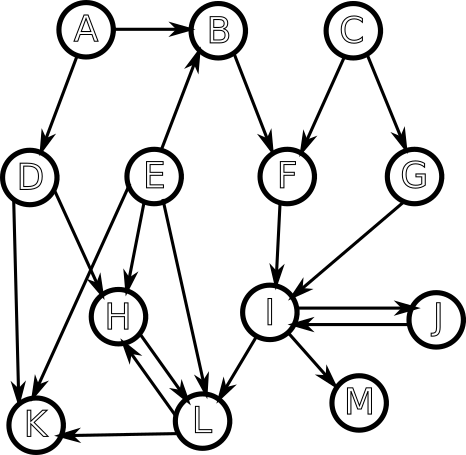
\includegraphics[width=\textwidth/2]{example-standard-graph}
  \caption[A standard graph]{An example of a standard graph. All edges represent directed, pairwise interactions between two nodes. Biologically, it is difficult to extract meaningful signaling pathway information from this graph, since protein complex formation and degradation is ambiguous.}
  \label{fig:example-standard-graph}
  \end{center}
\end{figure}

One area of cell-signaling that becomes particularly problematic in standard graphs is the formation, interaction, and destruction of protein complexes.  The easiest way that complexes can be represented in standard graphs is by creating a complete subgraph of all of the elements of the protein complex.  On their own, these complete subgraphs can yield useful information about the make-up of a protein complex, but once they begin interacting with other elements of the graph, the graph becomes much more complex, as all of the proteins in the complex must be represented independently.  In the case of interactions between multiple large complexes, it becomes the case that the standard graph representation of this interaction is a large complete subgraph that contains nodes for all of the proteins involved in either complex.  It is then computationally impossible to distinguish whether the entity being described by the subgraph is the interaction between multiple protein complexes, or simply one large complex that contains all of the components of both complexes.  Furthermore, since the complete subgraphs which represent complexes are undirected, it is difficult to deduce what the inputs or outputs of a biochemical reaction might be.\par

Another shortcoming of standard graphs in representing complex biological interactions is that there is no way in which to represent positive or negative regulation of interactions.  Since there is a standardized way in which edges interact with nodes, there is no way to differentiate types of interactions between nodes.  This poses a challenge when there are regulators or catalysts present that are necessary for a reaction, but are not part of the inputs or outputs of the reaction.  If regulators are to be included in a standard graph representation of a cell-signaling network, they become indistinguishable from any other types of interactions that are taking place.  This lack of specificity is problematic, as it treats all interactions as equal, and hides potentially useful information from the graph\footnote{The Reactome database is available for download as a standard graph, but it is not available as a directed graph. This means that we could not use their graphs as a standard graph comparison to ours.}.\par

To resolve the issues presented by standard graphs, we instead use a generalization called a \textit{hypergraph} that allows for the addition of more detail  and specificity within the data structure than standard graphs allow.  In particular, hypergraphs allow for both the representation of protein complexes in the form of \textit{hypernodes}, which we think of simply as a set of one or more nodes, and for the representation of complex, directed interactions that can have multiple inputs and outputs.  We represent these interactions with the use of \textit{hyperedges}, which define a set of one or more hypernodes\footnote{For simplicity, we treat each hypernode as a single node, in our treatment of signaling pathways, see Future Directions for more details. We will henceforth refer to all vertices in our hypergraphs as ``nodes" to avoide confusion.}.  Since a hyperedge may include more than two nodes, we gain the ability to represent both multi-protein interactions, as well as to define the notions of regulation on reactions. Figure \ref{fig:undirected_hypergraph} shows an example of an undirected hypergraph. Whereas a directed graph represents directed, pairwise interactions between only two vertices, we can use a \textit{directed hypergraph} to represent directed interactions between sets of vertices (nodes). \par

\begin{figure}[h]
  \begin{center}
    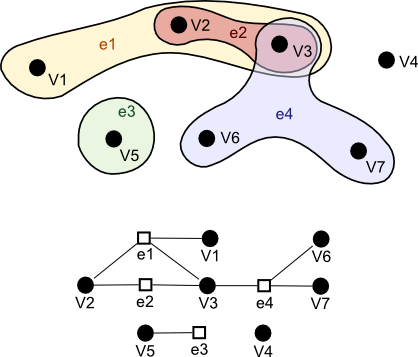
\includegraphics[width=\textwidth/2]{undirected_hypergraph}
  \caption[An example undirected hypergraph]{An example of an undirected hypergraph (\cite{sharpen}), where each edge is shown by a colored region, as well as the conversion of the hypergraph to a standard graph, where each hyperedge is shown as a node (white squares).}
  \label{fig:undirected_hypergraph}
  \end{center}
\end{figure}

\section{Directed Hypergraphs}

We formally define a directed hypergraph, $\mathcal{H}$, as a pair $(V,E)$, where $V$ is a finite set of vertices and $E \subseteq 2^V \times 2^V$ is a finite set of \textit{directed hyperedges} connecting members of $V$ such that, for every $e=(T(e),H(e)) \in E$, $T(e) \cap H(e) = \emptyset$, and $T(e)$, $H(e) \neq \emptyset$ (definition adapted from \cite{Gallo1993}).  We refer to $T(e)$ as the \textit{tail} of the hyperedge, and to $H(e)$ as the \textit{head} of the hyperedge.\par

\begin{figure}[thbp]
  \begin{center}
    \includegraphics[width=\textwidth/2]{example-hypergraph}
  \caption[An example directed hypergraph]{An example of the hypergraph, $\mathcal{H}=(V,E)$ that corresponds to the standard graph shown in Figure \ref{fig:example-standard-graph}. Note that each edge now contains more specific information about the propogation of a signal through the network. For this example, $V=\{A,B,...,M\}$ and each hyperedge is shown by a compound arrow, for example the edge whose tail is node $A$ and whose tail is nodes $B$ and $D$.}
  \label{fig:example-hypergraph}
  \end{center}
\end{figure}

It is important to note that a standard directed graph is a special case of a directed hypergraph.  This is the case if every node in the graph contains only one element, and if each hyperedgeedge has exactly one head element, and one tail element.  This has two important implications for algorithms that run on directed hypergraphs.  First, this means that there is no loss in functionality caused by using a hypergraph representation of a cell network, since anything that could be computed on a standard directed graph can be recreated exactly using the special case of the hypergraph. Secondly, this is important, because it means that anything that can be computed on a standard graph will be at least as computationally difficult to compute when generalized to a hypergraph.  In fact, we find that many tasks that are computationally easy on standard graphs become very difficult when generalized to hypergraphs (\cite{Ritz2014a}).\par

\begin{figure}[thbp]
  \begin{center}
    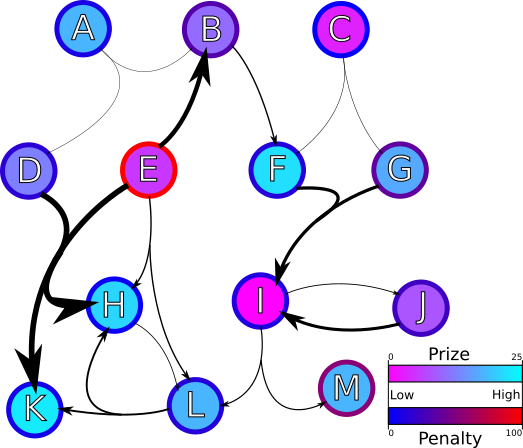
\includegraphics[width=\textwidth]{example-hypergraph-weighted}
  \caption[A weighted hypergraph]{The same hypergraph as in \ref{fig:example-hypergraph}, now weighted with node prizes (inner color) and root penalties (outer color). Edge thickness corresponds with edge weight. Intuitively, to find the PCSHN for this hypergraph, we want to find the subnetwork that maximizes the amount of blue, and minimizes the amount of both red nodes and thick lines.}
  \label{fig:example-hypergraph-weighted}
  \end{center}
\end{figure}

\section{Hyperpaths \& Connectivity}
In order to find the shortest route between two vertices, in a directed hypergraph, we define the notion of a \textit{directed hyperpath}, $\mathcal{P}$, on the directed hypergraph $\mathcal{H}$.  We think of a path, $\mathcal{P}$ from vertex $s$ to vertex $t$ as the list of vertices and hyperedges that one must pass through in order to traverse through the directed hypergraph from vertex $s$ to $t$. The existence of a hyperpath between two nodes encodes the notion of ``connectivity" between those nodes.  If a hyperpath exists between nodes $s$ and $t$, we say that they are \textit{connected}. This is a useful definition, because it allows us the notion of a \textit{connected hypergraph}, a hypergraph in which every node is connected by some hyperpath to every other node in the hypergraph.\par

\subsection{Directed Hyperpaths}

There are many ways in which we can define hyperpaths, but for the purposes of finding hypershrubs in directed hypergraphs, we must define a simple \textit{directed hyperpath} between nodes $s$ and $t$. We can think of a directed hyperpath $\mathcal{P}=s \cdot e_2 \cdot v_3 \cdots e_{n-1} \cdot t$ as an ordered list of nodes and edges, beginning with $s$ and ending with $t$ such that for any edge, $e_i$, in the path, $v_{i-1}$ is in the tail of $e_i$, and $v_{i+1}$ is in the head of $e_i$.\par

There are two types of hyperpaths that we find particularly interesting, as they give us the means to discuss very specific ways that signals can propagate. The first of these is a path that branches out from a one or more back-end nodes (Figure \ref{fig:BF-hyperpaths}). We call a hyperpath that branches out from a set of nodes a B-hyperpath (\cite{Gallo1993}). B-hyperpaths are especially interesting to biologists who seek to model signaling pathways, since a B-hyperpath represents all the products that can be reached from a given reactant (\cite{Ritz2014}).

\begin{figure}[!h]
  \begin{center}
    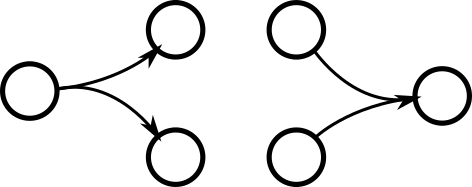
\includegraphics[width=\textwidth/2]{BF-hyperpaths}
  \caption[Simple B-Hypergrah and F-Hypergraph.]{\textit{left }A very simple example of a B-hyperpath. \textit{right }A simple example of an F-hyperpath. Note that even though both of these paths contain only one hyperedge, there may be longer hyperpaths, as long as they follow the same structure.}
  \label{fig:BF-hyperpaths}
  \end{center}
\end{figure}

The second type of hyperpath that we are interested in, F-hyperpaths, are very similar to B-hyperpaths, except that they are defined by a node on their front end (Figure \ref{fig:BF-hyperpaths}), and are made of hyperedges that lead into that edge. Biologically, this represents all of the reactions that can lead to a given product. Both of these types of hyperpaths will be formalized later, and they will be generalized as part of our definition of a hypershrub.

\chapter{Hypershrubs}

Recall that we are interested in finding meaningful signaling pathways in protein-protein interaction networks using hypergraph representations of the PPI networks. Remember as well that we want to use biological data to find subnetworks that capture the maximal amount of prize in the smallest network possible, much like in the Prize-Collecting Steiner problem. The first formulation is as an unweighted decision problem, where we seek to compute whether a certain substructure, with appropriate properties, is present in the network. In the second formulation, we include weights in the form of prizes and penalties and we seek to find a substructure that maximizes some optimization criterion computed from the weights.\par

Now, we will review the formulations of B- and F-hyperpaths, which are both concerned with single source-target pairs. From there, we will generalize these hyperpaths to include multiple targets. We first give a family of decision problems that seek a subhypergraph that includes certain targets and sources. We then relax the decision problem by formulating it as an optimization problem, seeking prize-rich targets and sources. We call these subnetworks \textit{hypershrubs}. Finally, we show how the optimization problem can coded as an integer linear program, allowing us to use existing tools, adapting them to find optimal hypershrubs.\par

\section{Hyperwalks}
In order build our formalization of B- and F-hyperpaths, we begin by defining \textit{hyperwalks}, an analog to a walk in a standard graph. We define a hyperwalk from $s$ to $t$ as a sequence of edges $\mathcal{W} \subseteq E$

\begin{align*}
  e_1 \cdot e_2 \cdot ... \cdot e_\ell
\end{align*}

of length $\ell$, where there is at least one shared vertex between $e_i$ and $e_{i+1}$ starting at $s$ and ending at $t$. We formalize this as: $H(e_i) \cap T(e_{i+1}) \neq \emptyset$ and $s \in T(e_1)$ and $t \in H(e_\ell)$. In other words, a hyperwalk is a series of ``hops" that one can make along directed hyperedges that take you from $s$ to $t$.\par

\subsection{B-connectivity}
For B-connectivity relative to a source, $s$, we consider a tree\footnote{Note that this is not to be confused with the mathematical structure.} of hyperedges emanating forward from $s$, with the condition that there be no ``loose tails," such as in Figure \ref{fig:B-Hypergraph}. More precisely, we define the set of \textit{outs} from $s$ in terms of a series of $\ell$ outward hops $\mathcal{O}_\ell(s)$ where:
\begin{align*}
  \mathcal{O}_0(s)&=\{s\}\\
  \mathcal{O}_{i+1}(s)&=\{u \,|\, u \in H(e) \text{ for some } e \text{ where } T(e) \subseteq \mathcal{O}_i(s)\}
\end{align*}
In English, this means that a node, $u$ is in $\mathcal{O}(s)$ under two conditions:
\begin{enumerate}
  \item{Node $u$ is $s$.}
  \item{Node $u$ is in the head of some edge, $e$ such that the entire tail of $e$ is in $\mathcal{O}(s)$.}
\end{enumerate}
We can now say that $s$ is \textit{B-connected} to some node $t$ if $t \in \mathcal{O}_h(s)$ for some $h \geq 0$. In other words, this means that $t$ is $h$ hops forward from $s$, and there is some walk from $s$ to $t$ for which there are no loose tails.\par

\begin{figure}[h]
  \begin{center}
    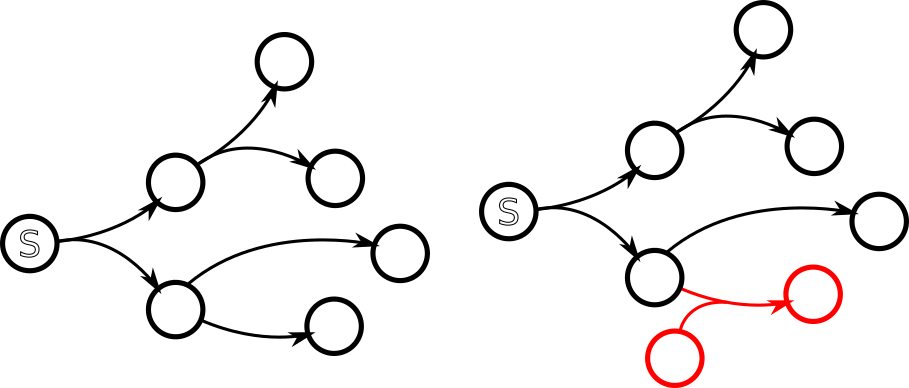
\includegraphics[width=\textwidth]{B-hypergraph}
  \caption[B-connectivity.]{\textit{left }A hypergraph $s$ is B-connected to all nodes, when a loose head is added \textit{right} $s$ is no longer B-connected to the head of that edge (shown in red).}
  \label{fig:B-Hypergraph}
  \end{center}
\end{figure}

\subsection{F-connectivity}
Similarly to B-connectivity, we can consider the set of nodes that ``funnel" into a given target node, $t$ without any loose heads. We therefore can use the same type of thinking to define the \textit{ins} to $t$ as a series of $\ell$ inward hops $\mathcal{I}_\ell(t)$ as follows:
\begin{align*}
  \mathcal{I}_0(t)&=\{t\}\\
  \mathcal{I}_{i+1}(t)&=\{v \,|\, v \in T(e) \text{ for some } e \text{ where } H(e) \subseteq \mathcal{I}_i(t)\}
\end{align*}
In English, this means that a node, $v$ is in $\mathcal{I}(t)$ under two conditions:
\begin{enumerate}
  \item{Node $v$ is $t$.}
  \item{Node $v$ is in the tail of some edge, $e$ such that the entire head of $e$ is in $\mathcal{I}(t)$.}
\end{enumerate}
Similarly, we can say that a node $s$ is F-connected to $t$ if $s \in \mathcal{I}_h(t)$ for some $h \geq 0$.

\section{B-, F-, \& BF-Hypershrubs}
In our formulation of B- and F-connectedness, we were focusing on the vertices that reach from or to a target. Instead, we might consider the edges that participate in $\mathcal{O}(s)$ or $\mathcal{I}(t)$. Consider the following, where $A \subseteq E$:

\begin{equation}
  H(A) = \bigcup_{e \in A} H(e)
\end{equation}
and
\begin{equation}
  T(A) = \bigcup_{e \in A} T(e)
\end{equation}
From this, we can also define the induced subset of nodes $V(A) = H(A) \cup T(A)$. From this, we also define the set of everything that is in the tail of some edge, but not in the heads of any hyperedges in $A$ as $D(A) = V(A) \setminus H(A)$. The set $D(A)$ represents the set of the \textit{induced roots} of $A$. Similarly, we find the \textit{induced leaves} of $A$ by defining $C(A) = V(A) \setminus T(A)$\footnote{Since roots being $D(A)$ and leaves being $C(A)$ are not very intuitive names, remember that roots go \textit{down}, and that leaves \textit{climb}.}. From these definitions, we can construct three definitions of Hypershrubs, \textit{B-Hypershrubs}, \textit{F-Hypershrubs}, and \textit{BF-Hypershrubs}. Intuitively, we think of a B-Hypershrub which strictly respects the backward set of nodes, an F-Hypershrub as one that strictly respects the forward set of nodes, and a BF-Hypershrub as one that strictly respects both sets of nodes. The names for these three types of hypershrubs is adapted from the naming convention for different types of hyperpaths (\cite{Gallo1993}). For all three of the hypershrubs, we begin with a hypergraph, $\mathcal{S}$, and two sets of nodes: a source set, $S$, and a sink set, $T$, where $S,T \subseteq V$. We now formulate three decision problems.\par

\subsection{B-Hypershrub}
We start by defining a hypershrub that, like a B-hyperpath, is defined by its back-end nodes:

\bigbreak

\hfill\begin{minipage}{\dimexpr\textwidth-2cm}
\paragraph{Given.}A directed hypergraph $\mathcal{H}=(V,E)$, and node sets $S$ and $T$.
\paragraph{Find.}$A \subseteq E$ subject to:
\begin{itemize}
  \item{$C(A) \subseteq T$}
  \item{$D(A) = S$}
\end{itemize}
\xdef\tpd{\the\prevdepth}
\end{minipage}
\bigbreak
We call the induced hypergraph of $A$ the B-Hypershrub, $\mathcal{B}$.\par

\subsection{F-Hypershrub}
Now, we formulate a decision problem that seeks a hypershrub defined by its forward elements:

\bigbreak

\hfill\begin{minipage}{\dimexpr\textwidth-2cm}
\paragraph{Given.}A directed hypergraph $\mathcal{H}=(V,E)$, and node sets $S$ and $T$.
\paragraph{Find.}$A \subseteq E$ subject to:
\begin{itemize}
  \item{$C(A) = T$}
  \item{$D(A) \subseteq S$}
\end{itemize}
\xdef\tpd{\the\prevdepth}
\end{minipage}
\bigbreak
We call the induced hypergraph of $A$ the F-Hypershrub, $\mathcal{F}$.\par

\subsection{BF-Hypershrub}
Finally, we formulate the most strict decision problem, as it inforces both the back and front sets of nodes:

\bigbreak

\hfill\begin{minipage}{\dimexpr\textwidth-2cm}
\paragraph{Given.}A directed hypergraph $\mathcal{H}=(V,E)$, and node sets $S$ and $T$.
\paragraph{Find.}$A \subseteq E$ subject to:
\begin{itemize}
  \item{$C(A) = T$}
  \item{$D(A) = S$}
\end{itemize}
\xdef\tpd{\the\prevdepth}
\end{minipage}
\bigbreak

We call the induced hypergraph of $A$ the BF-Hypershrub, $\mathcal{BF}$.\par

\begin{figure}[!h]
  \begin{center}
    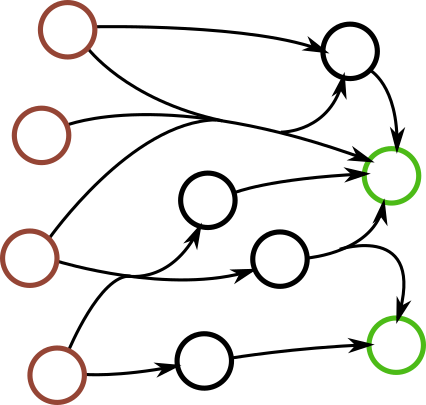
\includegraphics[width=3in]{BF-hypershrub}
  \caption[Hypershrub.]{A Hypershrub, with edge set $A$. The roots, $D(A)$ are shown in chestnut and the leaves, $C(A)$ in kelly green. All of the black nodes represent $H(A) \cap T(A)$.}
  \label{fig:BF-hypershrub}
  \end{center}
\end{figure}

One important piece to note is that we can easily reconstruct B, F, or BF-hyperpaths from $s$ to $t$ from their respective hypershrub generalizations by making $S=\{s\}$ and $T=\{t\}$. Furthermore, because we encode hypershrubs through the heads and tails of the included hyperedges, we implicitly know that there is always at least one hyperwalk from each $s \in S$ to some $t \in H(A)$, and from some $s \in T(A)$ to each $t \in T$. Finally, though this formulation does encode a hypershrub that is connected from its roots to its leaves, it does not necessarily encode a completely connected sub-hypernetwork, since these constraints could create two mutually exclusive hypershrubs from only one $S$ and one $T$.

\paragraph{Minimality.}In the formulations above we have few conditions on the hyperedge subset $A$. In some cases, we prefer some $A$ over others, namely ones with fewer hyperedges. That is to say, we might add aditional creteria to seek a subset $A$ of smallest size, with no cycles, and so forth. These are variations of the hypershrub decision problem stated above. From this, we say that the minimal B-hypershrub is one with the fewest hyperedges of all $A$ that satisfies the B-hypershrub property. Similarly, the minimal F-hypershrub and minimal BF-hypershrub are the ones with the fewest hyperedges of all $A$ that satisfy their respective hypershrub properties.\par

\section{Prize-Collecting Subhypernetworks}

When we are looking for a minimal BF-Hypershrub using empirical data, we often do not know what $S$ and $T$ are \textit{a priori}. To get around this, we instead try to determine a prize-collecting variant of the decision and optimization problem described above, so that we can determine a plausible set of roots and leaves that will define some BF-Hypershrub in a weighted hypergraph. We now can define the Prize-Collecting Subhypernetwork, $\mathcal{S} = (V^\prime,E^\prime)$, to be the set of nodes and hyperedges for which total vertex prizes are maximized, and total edge weights are minimized. We also try to minimize the cost that we give to each node for being present without any incoming hyperedge\footnote{In signaling pathways, this cost quantifies how likely or unlikely we consider it to be that a given reactant is present in the cell, agnostic to the reactions that caused it to be there.}.

To make our Prize-Collecting Subhypernetwork, $\mathcal{S}$, we begin with a parent hypergraph, $\mathcal{H} = (V,E)$, and a set of target nodes, $T$, such that $T \subseteq V$.  We refer to each node as some $v$ such that $v \in V$, and each edge is some $e$ such that $e \in E$.  When building $\mathcal{H}$, each hyperedge is assigned a weight, that is, a cost associated with including that edge in the solution hypergraph, $\mathcal{S}$.  We then assign each node in $\mathcal{H}$ a prize for being included in $\mathcal{S}$. We can now define the \textit{weighted subhypernetwork problem} as an optimization question:\par
\bigbreak

\hfill\begin{minipage}{\dimexpr\textwidth-2cm}
\paragraph{Given.}A directed hypergraph $\mathcal{H}=(V,E)$, and weight functions $g:V \rightarrow \mathbb{Z}^+$ and $c:E \rightarrow \mathbb{Z}^+$.
\paragraph{Find.}$A \subseteq E$ which minimizes:
\begin{align*}
  o(A) = \sum_{v \in V(A)}g(v) - \sum_{e \in A}c(v)
\end{align*}
%\xdef\tpd{\the\prevdepth}
\end{minipage}
\bigbreak
In this formulation, the first part of the objective function codes for ``reaching" for higher prize nodes, and the second part codes for ``trimming back" based on edge cost. This problem is, in some ways, analogous to the Prize-Collecting Steiner tree optimization problem. We can add further detail to this problem by adding two new parts to the optimization problem. We call this formulation the \textit{weighted subhypernetwork problem with root and leaf penalties}. We precisely define this optimization question as:\par
\bigbreak

\hfill\begin{minipage}{\dimexpr\textwidth-2cm}
\paragraph{Given.}A directed hypergraph $\mathcal{H}=(V,E)$, weight functions $g:V \rightarrow \mathbb{Z}^+$ and $c:E \rightarrow \mathbb{Z}^+$, and penalty functions $h:V \rightarrow \mathbb{Z}^+$ and $\ell:V \rightarrow \mathbb{Z}^+$.
\paragraph{Find.}$A \subseteq E$ which minimizes:
\begin{align*}
  o(A) = \sum_{v \in V(A)}g(v) - \sum_{e \in A}c(v) - \sum_{v \in D(A)}h(v) - \sum_{v \in C(A)}\ell(v)
\end{align*}
%\xdef\tpd{\the\prevdepth}
\end{minipage}
\bigbreak
In this new formulation, we add two new parts to the objective function. The first penalizes nodes for being present in the output graph if they have no incoming hyperedges, that is, they are a dangling root node. Similarly, the second new part of the objective function penalizes nodes for being dangling leaves, ones with no outgoing hyperedges in the solution.

\section{Implementation as an Integer Linear Program}

To start our implementation, we begin by looking backwards through a hypergraph from a set of target nodes, $T$. We begin in this way because, in PPI data, downstream nodes are often more easily inferred using empirical data such as gene expression, since changes in the expression of some genes is the ultimate output of cell signaling pathways.

Given an input hypergraph $\mathcal{H}=(V,E)$, and a set of target nodes, $T$, we construct a subhypernetwork, $\mathcal{S}= (V^\prime,E^\prime)$, where $V^\prime \subseteq V$ and $E^\prime \subseteq E$.  We build $\mathcal{S}$ using an ILP which encodes the definition of a subhypernetwork.  In order to accomplish this, we define three indicator variables, $\alpha_v$, $\alpha_e$, and $\delta_v$, where $v$ and $e$ are nodes or hyperedges in $\mathcal{H}$.  If node $x$ is in the solution of the ILP, $\alpha_v$ will have a value of 1, otherwise it will be equal to 0.  Similarly, if edge $e$ is present in the solution, $\alpha_e$ will take a value of 1. The value of $\delta_v$ will be determined by whether a node is a root in the solution, 1 if it is, 0 if not.\par

We find the subhypernetwork $\mathcal{S}$ by optimizing the function:

\begin{equation} \label{eq:ilpsum}
 \argmax_{\alpha, \delta} \sum_{v \in V} g_v \alpha_v - \sum_{e \in E} c_e \alpha_e - \sum_{v \in V} h_v \delta_v
\end{equation}

Subject to the set of linear constraints:

\begin{align}
 \alpha_v \geq 1 \qquad\qquad &\forall\; v \in T\label{eq:ilpT}\\
 \sum_{v \in H(e)} \alpha_v \geq \lvert H(e)\rvert \alpha_e \qquad\qquad &\forall\; e \in E\label{eq:ilpinchead}\\
 \sum_{v \in T(e)} \alpha_v \geq \lvert T(e)\rvert \alpha_e\qquad\qquad &\forall\; e \in E\label{eq:ilpinctail}\\
 \delta_v \leq \alpha_v \qquad\qquad &\forall\; v \in V\label{eq:ilpdang1}\\
 \delta_v \geq \alpha_{v} - \sum_{e:v \in H(e)} \alpha_e \qquad\qquad &\forall\; v \in V\label{eq:ilpdang2}%
\end{align}%


Here, the objective function \eqref{eq:ilpsum} tries combinations of nodes ($\alpha_v$), edges ($\alpha_e$), and root nodes ($\delta_v$) that maximize the sums of node prizes ($g_v$), minimize the sums of edge costs ($c_e$), and minimize the sums of root penalties ($h_v$). Constraint \eqref{eq:ilpT} encodes that every target node in $T$ is in the solution, $\mathcal{S}$.  Constraints \eqref{eq:ilpinchead} and \eqref{eq:ilpinctail} ensure that if an edge is in $\mathcal{S}$, any nodes incident on that edge (i.e. in the head or tail of that edge) will also be in $\mathcal{S}$.  Finally, constraints \eqref{eq:ilpdang1} and \eqref{eq:ilpdang2} encode the ability for nodes to dangle if they do not have an incoming edge. To illustrate what each of these constraints does in more detail, we will construct a simple example, and examine each constraint within that example.\par

\begin{figure}[th]
  \begin{minipage}[b]{0.30\linewidth}
    \centering
    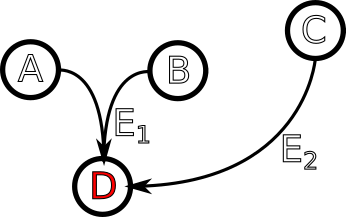
\includegraphics[width=\linewidth]{dummy-before}
    \par\vspace{0pt}
  \end{minipage}%
  \begin{minipage}[b]{0.30\linewidth}
    \centering%
    \begin{tabular}{ |l|l|l| }%
      \hline%
      \multicolumn{3}{|c|}{Nodes} \\%
      \hline \hline
      Node & $g_v$ &  $h_v$ \\ \hline%
      $A$ & 10 &  1\\ \hline%
      $B$ & 10 &  1\\ \hline%
      $C$ & 1 &  10\\ \hline%
      $D$ & 10 &  10\\ \hline%
    \end{tabular}%
    \par\vspace{0pt}
  \end{minipage}
  \begin{minipage}[b]{0.30\linewidth}
    \centering%
    \begin{tabular}{ |l|l| }%
      \hline%
      \multicolumn{2}{|c|}{Edges} \\%
      \hline \hline
      Edge & $c_e$ \\ \hline%
      $E_1$ & 1 \\ \hline%
      $E_2$ & 10 \\ \hline%
    \end{tabular}%
    \par\vspace{0pt}
  \end{minipage}
\caption[A small hypergraph, with node and edge data]{A simple hypergraph, and its associated node and edge weights.}
\label{fig:dummy-before}
\end{figure}

\paragraph{Example.}Consider the hypergraph shown in Figure \ref{fig:dummy-before}. For this hypergraph, the PCSHN that comes from this graph should consist of nodes $A$, $B$, and $D$, as well as hyperedge $E_1$. This is obvious, since nodes $A$ and $B$, which will be a root in the solution, both have low root penalties and high prizes, while node $C$ has a very large root penalty relative to its prize. Similarly, $E_1$ has a relatively low cost, whereas $E_2$ has a very high cost. Finally, $D$ is considered a target, in this case, and is therefore automatically included in the solution. Knowing what the solution should be, we can use this hypergraph to demonstrate the effect of each linear constraint in our ILP.\par

\begin{table}[!h]
\begin{center}
  \label{tab:obj_values_dummy}
  \caption[Objective values of dummy hypergraph.]{All of the possible solutions that satisfy all necessary linear constraints, and their corresponding objective values. We see that the induced subgraph from $E_1$ yields the optimal solution.}
\begin{tabular}{ |l|l|l| }%
  \hline%
  \multicolumn{3}{|c|}{Subgraphs} \\%
  \hline \hline
  $V$ & $E$ & Objective Value \\ \hline%
  $A,B,D$ & $E_1$ & 27 \\ \hline%
  $C,D$ & $E_2$ & -9 \\ \hline%
  $A,B,C,D$ & $E_1,E_2$ & -2 \\ \hline%
\end{tabular}%
\end{center}
\end{table}

We now know that, for the optimal PCSHN, $\alpha_A$, $\alpha_B$, $\alpha_D$, and $\alpha_{E_1}$ are all equal to 1 (that is, they are included in the solution), and $\alpha_C$ and $\alpha_{E_2}$ are equal 0. Additionally, we know that in this solution $A$ and $B$ are root nodes, therefore $\delta_A$ and $\delta_B$ are both 1, and $\delta_C$ and $\delta_D$ are both 0. Finally, we are given that $D$ is a target node, hence $T=\{D\}$.\par

First let us look at the objective function, Formula \eqref{eq:ilpsum}. We can call each of the three sums included the equation which calculate the total node prizes, edge costs, and root penalties $\Xi$, $\Phi$, and $\Psi$, respectively. Given the values of $\alpha_v$, $\alpha_e$, and $\delta_v$ that we know should yield the PCSHN, we find:
\begin{gather*}
 \Xi = 30\\
 \Phi = 1\\
 \Psi = 2\\
 \implies \Xi - \Phi - \Psi = 27\\
\end{gather*}%
If $C$ or $E_2$ were to be added, or any node or edge were removed from the PCSHN, the total value of the objective function would decrease, therefore yielding a suboptimal solution to the ILP.\par

Now, we can begin to look at how each linear constraint governs the behavior of the ILP. Let's begin with constraint \eqref{eq:ilpT}. For our hypergraph, $T$ only has one element, $D$, constraint \eqref{eq:ilpT} only needs to be checked for one node. We know that $\alpha_D = 1$, therefore constraint \eqref{eq:ilpT} simplifies to:
\begin{align*}
  \alpha_D &\geq 1\\
\end{align*}
We see that constraint \eqref{eq:ilpT} holds for all $v$ in $T$, therefore we know that all members of the target set are included in the PCSHN.\par

Next, we can look at constraints \eqref{eq:ilpinchead} and \eqref{eq:ilpinctail}. Since these constraints are the same, except for whether they are concerned with the head or tail of a hyperedge, we can evaluate the effect of only constraint \eqref{eq:ilpinchead}, and assume that constraint \eqref{eq:ilpinctail} works in the same way. To assess this constraint, we must see how if the inequality holds for all edges in the hypergraph. We begin by looking at $E_1$. We know that $H({E_1})=D$, and that $\lvert H(e) \rvert = 1$, therefore we can check:
\begin{align*}
  \alpha_D &\geq 1 \bullet \alpha_{E_1}\\
\end{align*}%
So, we see that constraint \eqref{eq:ilpinchead} holds for $E_1$. Now, we can check for $E_2$ (whose head is also only $D$):
\begin{align*}
  \alpha_D &\geq 1 \bullet \alpha{E_2}\\
\end{align*}%
We see that this inequality also holds. This means that, since the inequality holds for all hyperedges, that for every edge in the hypergraph, its head is also included in the hypergraph. We can easily extend this to see that \eqref{eq:ilpinctail} enforces the same for the tails of every hyperedge.\par

Finally, we can look at the three constraints that allow nodes to be a root: constraints \eqref{eq:ilpdang1} and \eqref{eq:ilpdang2}. First, we look at constraint \eqref{eq:ilpdang1}:
\begin{alignat*}{4}
  \delta_A &\leq \alpha_A \qquad \delta_B &&\leq \alpha_B \qquad \delta_C &&\leq \alpha_C \qquad \delta_D &&\leq \alpha_D\\
\end{alignat*}%
Now that we see that constraint \eqref{eq:ilpdang1} holds for all nodes in the PCSHN, we can look at \ref{eq:ilpdang2}. This constraint is trivial for every node in the hypergraph other than $D$, since it is the only node in the head of any hyperedges:
\begin{align*}
 \delta_D \geq \alpha_{D} - \alpha_{E_1} - \alpha_{E_2}\\
\end{align*}%


\section{Roots and Leaves Problem}

When we implement the ILP in a more complex hypergraph, such as the hypergraph shown in Figure \ref{fig:example-hypergraph-weighted}, we find that it creates a hypergraph that consists of multiple smaller hypergraphs (Figure \ref{fig:example-hypergraph-weighted-after-ILP}), rather than a continuous subnetwork. Our original implementation ends up returning a group of disconnected hypergraphs that represent regions with high prize to edge/root cost ratios, separated by gaps where the parent hypergraph had regions of low prize to edge/root cost ratios. While this result is interesting in itself, it will not necessarily create a solution that is biologically interesting once we begin looking for PCSHNs in pathway signaling data.\par

\begin{figure}[hp]
  \begin{center}
    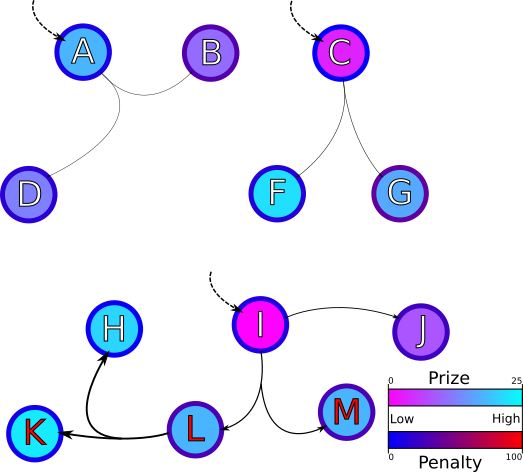
\includegraphics[width=\textwidth]{example-hypergraph-weighted-after-ILP}
  \caption[Output from ILP with disconnected sub-hypergraphs]{The output of our ILP, when it is run on the hypergraph shown in Figure \ref{fig:example-hypergraph-weighted}. The dashed arrows indicate a root node.}
  \label{fig:example-hypergraph-weighted-after-ILP}
  \end{center}
\end{figure}

Our new goal is to find a way to connect regions that would be disconnected in the original formulation of the PCSHN. In doing so, we have two cases that may exist: the region between sub-hypernetworks is prize-rich or it is prize-poor. If the region is prize-rich, we would want to connect the two regions throuh that region to construct a larger PCSHN that explains the lowest cost connecting region. If the region is prize-poor, on the other hand, we would rather have the less valuable sub-hypernetwork to be left out of the final PCSHN, since the cost of reaching it would not justify the prize that the sub-hypernetwork contained. Additionally, we need to consider the case where there is no way to get from one sub-hypernetwork to another sub-hypernetwork, we will allow both to be present in the final solution.\par

To accomplish these goals, we use the set of nodes that either have no incoming or outgoing hyperedges in the solution: the roots and leaves. We are only concerned with these dangly nodes, and not with the inner nodes because we want to keep the same topology that is generated by the original formulation, and not be concerned with any hyperedges that may connect the middle parts of sub-hypernetworks, but whose prices are too high to justify being included in the solution. When we think of this biologically, it means that we do not want to force including a reaction in the solution just because its reactants and products are present elsewhere in the solution, if there are already lower cost explanations for why they are present.\par

To fix this new problem, we must incorporate the notion of hyperpaths and connectedness to our implementation of the PCSHN, as well as define the class of leaf variables in our formulation. Additionally, we must construct a matrix of whether or not there exists a hyperpath of any kind between every pair of nodes in $\mathcal{H}$. As such, we adopt the notation $\iota_v$, as a binary variable that indicates whether node $v$ is a leaf in the solution. Furthermore, we introduce the binary variable $\mathcal{P}(u,v)$ to indicate whether or not a hyperpath exists from $u$ to $v$. From this, we simply say that if there exists a hyperpath from node $s$ to $t$, then either $s$ cannot be a leaf or $t$ cannot be a root (i.e. $\mathcal{P}(u,v)\implies\neg(\delta_u\wedge\iota_v)$).\par

\paragraph{Implementation in the ILP.}To add this change to the ILP for the PCSHN it is necessary to implement three new linear constraints, as well as the two new sets of variables described already, $\iota$ and $\mathcal{P}$. It is important to note that, in a hypergraph with $n$ vertices, this will add $n$ new $\iota$ variables, and $n^2$ new $\mathcal{P}$ constraints, since every pairwise combination of vertices $(s,t)$ must be checked to see if there is a hyperpath from $s$ to $t$.

We introduce linear constraints:

\begin{align}
 \iota_v \leq \alpha_v \qquad\qquad &\forall\; v \in V\label{eq:dc1}\\
 \iota_v \geq \alpha_{v} - \sum_{e:v \in T(e)} \alpha_e \qquad\qquad &\forall\; v \in V\label{eq:dc2}\\
 2 - \delta_u - \iota_v \leq \mathcal{P}_{u,v} \qquad\qquad &\forall\; u,v \in V\label{eq:dc3}%
\end{align}%

Similarly to in the original constraint \eqref{eq:ilpdang1}, constraint \eqref{eq:dc1} ensures that all nodes which are considered leaves must be present in the solution. Additionally, constraint \eqref{eq:dc2} follows the same form as constraint \eqref{eq:ilpdang2}, only it now applies to edges for which the node of interest is in the tail, rather than the head. These two constraints enforce the labeling of nodes that do not have an outgoing hyperedge as leaves. Constraint \eqref{eq:dc3} is where we encode that that if a path exits from $u$ to $v$, then either $u$ cannot be a leaf, or $v$ cannot be a root, in the PCSHN. When we implement these three linear constraints, along with the existing set in the hypergraph from Figure \ref{fig:example-hypergraph-weighted}, we find a new solution, as shown in Figure \ref{fig:example-hypergraph-weighted_DC}.

\begin{figure}[hp]
  \begin{center}
    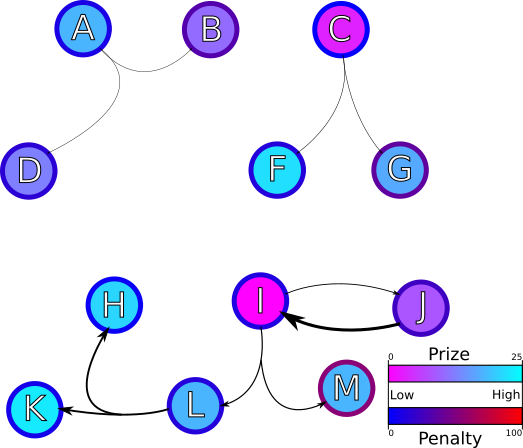
\includegraphics[width=\textwidth]{example-hypergraph-weighted_DC}
  \caption[Output from ILP after Roots and Leaves.]{The output of our ILP, when it is run on the hypergraph shown in Figure \ref{fig:example-hypergraph-weighted}, also taking the Roots and Leaves problem into account.}
  \label{fig:example-hypergraph-weighted_DC}
  \end{center}
\end{figure}

\paragraph{Running Time.}It is important to note at this point that, because the number of variables and constraints in the ILP now quadratic with respect to the number of nodes in the original hypergraph, the amount of time that the ILP will take to solve will increase rapidly with the number of nodes. To this end, even the time to build the \texttt{.lp} files that are the input of the ILP solver is non-trivial on large datasets. This is illustrated in the table below.

\begin{table}[!h]
\begin{center}
  \label{tab:build_lp_runtimes}
  \caption[Runtimes of ``build lp" programs.]{Four datasets of increasing size, and how long they take to be converted into \textit{.lp} files using both the original formulation (\textit{blp}) and the formulation that takes into account the roots and leaves problem (\textit{blprl}). Input files are the dummy hypergraph used in \ref{fig:dummy-before}, the example hypergraph from \ref{fig:example-hypergraph-weighted}, the Hedgehog signaling pathway, and the entire Reactome database for \textit{A. thaliana}. All times are in seconds.}
\begin{tabular}{ |l||l|l|l|l|l|l| }%
  \hline%
  Hypergraph & Nodes & Edges & Time(\textit{blp}) & Time(\textit{blprl}) & Lines(\textit{blp}) & Lines(\textit{blprl}) \\%
  \hline \hline
  dummy & 4 & 2 & 0.00066 & 0.00095 & 30 & 86 \\ \hline%
  ex & 13 & 12 & 0.00115 & 0.00274 & 100 & 633 \\ \hline%
  Hh & 413 & 82 & 0.0183 & 1.464 & 1,904 & 514,437  \\ \hline%
\end{tabular}%
\end{center}
\end{table}


\chapter{Implementation in Signaling by Hedgehog}

To analyze how the Prize-Collecting Subhypernetwork formulation performs on real data, we implemented it in the Hedgehog signaling pathway that we discussed earlier. Our goal was to reconstruct sub-pathways from the Hh signaling pathway that represent dysregulated subcomponents between patients with basal cell carcinoma an healthy patients.

\section{Inputs to Prize-Collecting Subhypernetwork}

  \subsection{Network Construction}
  In order to construct directed signaling hypergraphs of biological pathways, we use pathway data from preexisting, curated protein-protein interaction networks, available publically. For this, pathway signaling information was downloaded from the curated Reactome pathway database (\cite{Croft2014}, \cite{Milacic2012}), and parsed using a Java script (\cite{AnnaCorrespondence}) into two flat files containing node and edge information necessary to construct the hypergraph (See Appendix A).\par

  The networks generated from the Reactome database specify each complex as a combination of one or more proteins. For simplicity, each complex was ``converted" into a regular node for the purpose of algorithm implementation, and the components' information was saved so that they could be reconstructed \textit{post hoc}. Additionally, each hyperedge contained information about whether the reaction that it represented was regulated either positively or negatively by one or more nodes. Positive regulators were added to the tail of their respective hyperedges, since they are assumed to be necessary reactants for the edge, and should therefore be considered part of the signaling network. Negative regulators, on the other hand, were excluded from the flat files, since the way that they act on reactions poses an interesting problem in modeling, since the current definition of PCSHN assumes that all node prizes and edge weights are positive (see Future Directions).\par

  From the edge files, hypergraphs were constructed using the Hypergraph Algorithms Package (HALP, \cite{halp}). Edge files gave enough information to create induced hypergraphs, which were then weighted based on information stored in node files. The hypergraph representation of the Hh pathway contained 82 unique hyperedges, representative of biological reactions, and 413 unique nodes, each representative of a protein, complex, or small molecule. This means that there are, on average, 5 nodes incident on each hyperedge in the Hh pathway.\par

  \subsection{Human Cancer Data}

  To weight our hypergraph, we used a dataset available publically on the Gene Expression Omnibus (GEO), a database curated by the NCBI. The dataset analyzed contained gene expression from 26 patients with non-melanoma skin cancers divided into three groups (\cite{Jee2015}): sixteen BCC, ten SCC, and four Normal\footnote{For basal cell carcinoma, squamous cell carcinoma, and healthy patients, respectively.}. There were samples from both male and female patients. For our analysis, we excluded SCC samples, since dysregulations in our pathway of interest have been more heavily implicated with BCC. Additionally, the current ILP implementation has been designed with differential expression between two sample types in mind, so using three types could cause unexpected results that we are not prepared to analyze at this time.\par

   For statistical analysis of differential expression, we used the GEO2R interactive web tool (\cite{Davis2007}), available through NCBI. We used this tool to compute the adjusted $p$-value corrected by Benjamini \& Hochberg false discovery rate (FDR) and log fold change between genes from the two different samples. From this differential expression was calculated for 47,324 unique Illumina IDs. Of these, 31,072 had valid gene names that could be mapped to UniprotKB identifiers (\cite{TheUniProtConsortium2014}), which themselves were mapped to Reactome IDs and used to apply prizes to the Hh hypergraph.\par

   \section{Network Weighting}

   \subsection{Differential Expression-Based Weighting}

   Using gene expression data, 268 of the 413 nodes were assigned prizes equal to the negative log of their FDR. We chose this metric for giving prizes to nodes since it quantifies the likelihood that a particular gene is differentially expressed between the two tissue samples, regardless of whether it was up or down regulated. Though this is a relatively coarse way of weighting nodes, it gave us a way to look at emergent hypershrubs based on high confidence changes. We weight complexes by assigning their respective node a prize equal to the minimum prize among all nodes present in the complex.\par

   \subsection{Default Parameters}

   For the implementation PCSHN to create meaninful subnetworks, it is important that the parent hypergraph have a meaningful, biologically informed weighting scheme applied. However, it is often the case that data are difficult to acquire and add to the hypergraph, so simple default settings were first applied to each parameter. Each hyperedge was given a default value of 1, for simplicity.\par

   By using gene expression data, we were able to assign prizes to roughly half of the nodes in our hypergraph. Recall that our weighting scheme assigned prizes proportional to our confidence that there is differential expression between two samples. Because of this, we seek to assign prizes to the set of nodes that recieved no biological weighting, so that they are not unnecessarily penalized for us lacking data on their differential expression. If we were to give all unweighted nodes a default prize of zero, for instance, our formulation would treat those nodes as though we had zero confidence that they were implicated in dysregulated pathways. Similarly, we seek a default root penalty to apply to all nodes that sufficiently large to make reconstucted subhypernetworks meaningful, but not so strict that the subhypernetworks are too small to be informative. We test 5 values of default prizes, and 5 values of default root penalties (See Section 4.3.1).\par

   \section{Results on Hedgehog Signaling}

   \subsection{Original Formulation}

   We originally examined the output of our original formulation of the weighted subhypernetwork problem, without the roots and leaves constraint. We began here to determine if our less constrained version yielded any results and, if so, to get a baseline output to which we could compare our implementation of the weighted subhypernetwork problem with root and leaf penalties. By doing this, we could compare to see if the more complex version actually makes meaningful changes to the output, or if it simply added more complexity to generate the same or similar result.

   \subsubsection{Default Parameter Robustness}

   To find the optimal default node prize and penalty, we first tested a range of possible values for each parameter to find the largest subnetwork, as shown in Figure \ref{fig:Hh_nodes} and Figure \ref{fig:Hh_hyperedges} using our initial (without Roots and Leaves problem) formulation. We analyzed default settings of 0, 0.75, 1, 2.5, 5, 7.5, 10, and 100 for both the node prizes and root penalties. \par

   Our analysis of different node prizes and root penalties (shown in Figure \ref{fig:Hh_nodes} and Figure \ref{fig:Hh_hyperedges}) helps confirm that our integer linear program was performing as expected in several ways. We find that, in the case where root penalties are equal to zero, there were no hyperedges present in the solution. This makes sense because, with no root penalty, there is no disadvantage to every node that is included being a ``singleton" with no incoming or outgoing hyperedges, since all hyperedges can do is lower the total objective value. This pattern is also present, to a lesser extent in the cases where the default penalty is 0.75 or 1, which is very low compared to the other options. \par

   \begin{figure}
     \centering
     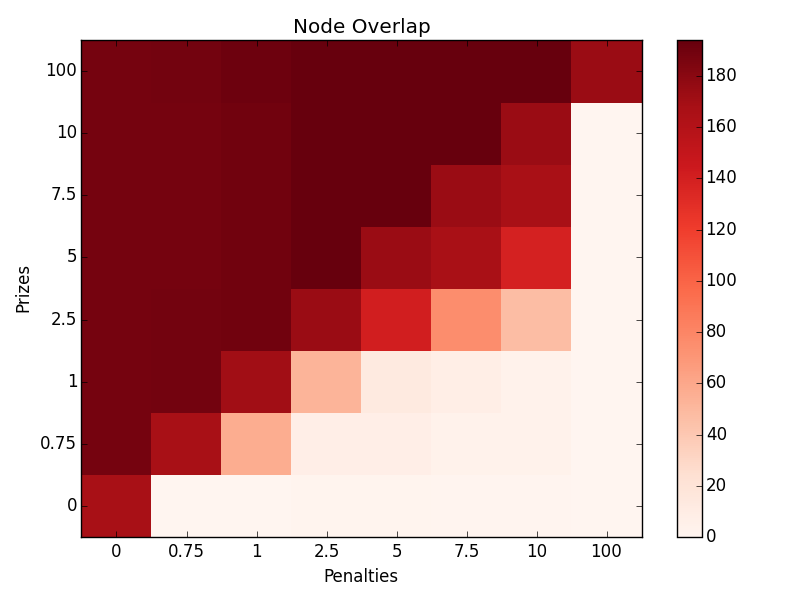
\includegraphics[width=0.8\linewidth]{Hh_nodes}
     \caption{The number of nodes as a function of default node prize and root penalty included in the solution to the weighted subhypernetwork problem. }
     \label{fig:Hh_nodes}
   \end{figure}%

   \begin{figure}
     \centering
     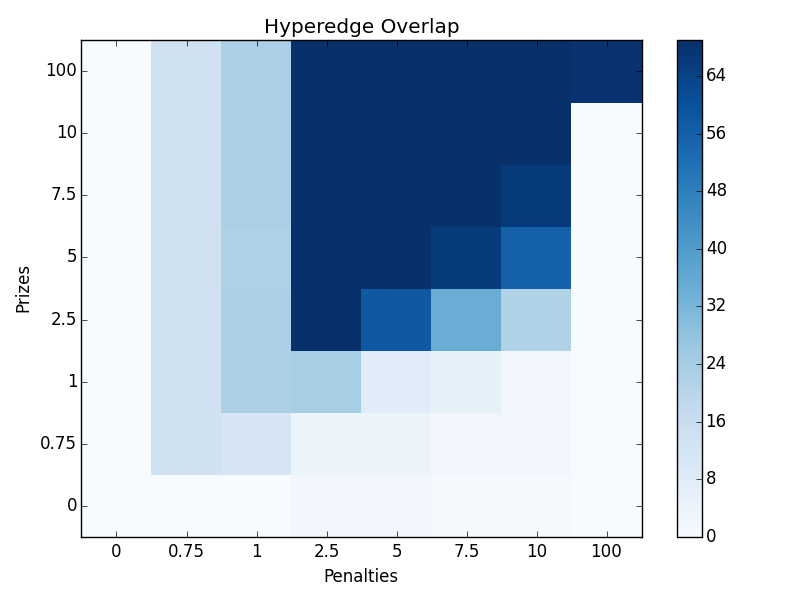
\includegraphics[width=0.8\linewidth]{Hh_hyperedges}
     \caption{The number of hyperedges as a function of default node prize and root penalty included in the solution to the weighted subhypernetwork problem.}
     \label{fig:Hh_hyperedges}
   \end{figure}

   Another pattern that we find is that the total number of nodes remains fairly constant across all cases where the default prize and root penalty are equal. This indicates that there exists some subset of the nodes and hyperedges whose total assigned prize, not default prize, justifies inclusion in the solution. Similarly, the upper left portion of both figures, which corresponds to prizes that are greater than penalties, is very dense with nodes, as expected. We see this pattern as well in the number of hyperedges, from a default penalty of 2.5 and greater, indicating that 2.5 is roughly the minimum pentalty for which reasonably large subnetworks will be reconstructed.\par

   The final interesting feature that we find in these heatmaps is the ``bulge" that exists in both figures where the prizes range from 2.5 to 5 and penalties range from 7.5 to 10. Because this region does not follow the expected patterns that we discussed above, it is the region that we selected from when choosing our default parameters. We did this because the changes that caused this area to stand out may be indicative of interesting phenomena in the hypergraphs.\par

   Using this method, we chose default parameters of 2.5 for node prizes and 7.5 for node penalties. These values are indicative of a default prize on nodes that did not have a biologically informed prize that is one third of the average biological prize, and a node penalty equal to the average node prize for the biologically informed nodes.\par

   \subsubsection{Network Fragmentation}

   Following the implementation without the Roots and Leaves problem, we found that the output was highly fragmented, containing many disconnected subhypernetworks. Upon analyzing the Prize-Collecting Subhypernetwork produced by our program, we find that the solution contained 44 hyperedges and 99 nodes. Of these nodes, 68 were Proteins. Additionally, we found that the resulting subhypernetwork was very disconnected, with one third of nodes present in the solution being roots. To lower this amount of disconnectedness, we used the Roots and Leaves implementation, with the same default node prize and penalty (2.5 and 7.5, respectively). \par

   \subsection{Roots \& Leaves Formulation}

   Following our implementation of the weighted subhypernetwork problem with root and leaf penalties, we found a much smaller set of root and leaf nodes, in a hypernetwork of similar size, implying a more connected subhypernetwork.\par

   \subsubsection{Network Fragmentation}

   Upon implementation of the Roots and Leaves version of the integer linear program. In the new solution, there were 44 hyperedges. The output of this also yielded 35 proteins, of which 7 were roots, and 4 were leaves. Furthermore, 36 complexes and 11 small molecules were present in the solution. Among the complexes, 6 were roots and 8 were leaves. Similarly, the small molecules included 8 roots and 5 leaves. In total, this gave us a subhypernetwork with 82 nodes. This subhypernetwork, though similar in total size, has much fewer root and leaf nodes relative to in the first formulation, meaning that it is a more connected solution.\par

   \subsubsection{Reconstructed Pathways}

   To analyze this subhypernetwork, we looked for any signaling pathways that were reconstructed in the hypergraph from start to finish. Since the output hypergraph was still relativly large compared to our examples, we restricted our analysis to one subcomponent of the Hedgehog signaling pathway, known as the \textit{Hedgehog `on' state} that accounts for approximately one third of the reactions in the Hh signaling pathway. Using this, we were able to search for any nodes that were roots or leaves in the solution, which were present in this pathway. Similarly, we were able to look at the biochemical reactions in the \textit{Hedgehog `on' state}, to determine if those reactions connected the roots and leaves that we found.\par

   One reaction that we find in this solution is the path from Kif7, SUFU, and Gli2 molecules and the EVC:EVC2 complex to yield Gli2 and SUFU. This particular pathway involves three hyperedges, two cases of positive regulation, and eight total nodes, shown in Figure \ref{fig:Hh-signaling-output}. As a reminder of our discussion on the Hedgehog signaling pathway, Gli2 is a transcription factor that marks one of the endpoints of Hh signaling. Kif7 is a kinesin that is known for regulating the Hedgehog signaling pathway and controling localization of SUFU:Gli2 to the ciliary membrane. SUFU is a kinesin-binding protein that is known to down-regulate Gli2-mediated activation of genes. Finally, EVC and EVC2 are proteins that exist in the downstream Hedgehog-Smoothened signaling pathway that are known to regulate signaling by Hedgehog (\cite{TheUniProtConsortium2014}).\par

    \begin{figure}[!h]
      \begin{center}
        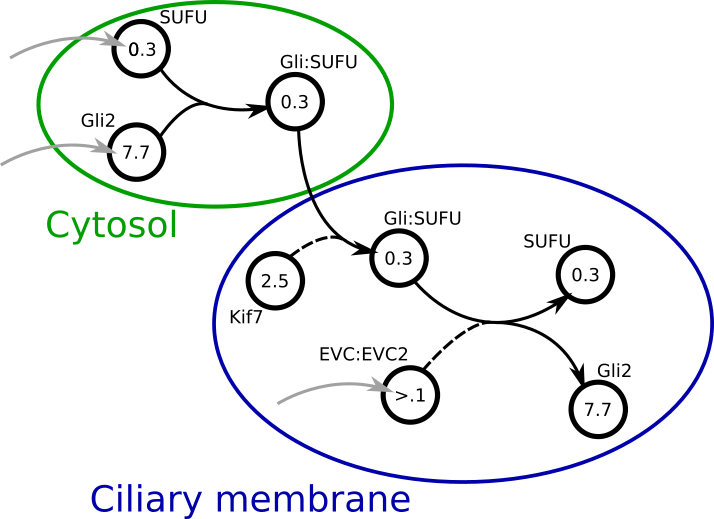
\includegraphics[width=\textwidth]{Hh-signaling-output}
      \caption[B-connectivity.]{A subset of the output hypergraph from out Roots and Leaves implementation of the weighted subhypernetwork ILP. Gray hyperedges show that the the node was in the head or tail of some other hyperedges in the solution, outside of the \textit{Hedgehog `on' state}. Node prizes are shown inside of the nodes.}
      \label{fig:Hh-signaling-output}
      \end{center}
    \end{figure}

    Biologically, this corresponds to the movement of SUFU and Gli2 from the cytosol to the ciliary membrane, assisted by Kif7 and EVC:EVC2. First, SUFU and Gli2 bind together to form the SUFU:Gli2 complex. Then Kif7 assists the complex in to the ciliary membrane. Finally, EVC:EVC2 assists in the dismantling of the SUFU:Gli2 complex, helping to divert Gli2 from the degradation pathway, allowing for Gli2 to localize to the nucleus and cause transcriptional changes (\cite{Humke2010}). This particular part of the Hh pathway has been implicated in the up-regulation of Hedgehog signaling (\cite{Tukachinsky2010}). Since upregulation of the Hh signaling pathway has been connected to increased risk for BCC, this may be one mechanism that could be a predictor for increased risk of BCC.\par

    The pathway that we found contained the only root that was present in the \textit{Hedgehog `on' state}, as well as two of the three leaves that were present\footnote{Interestingly, the only other leaf that was present in the \textit{Hedgehog `on' state} was Ptch1, the receptor that we originally discussed in our description of signaling by Hedgehog.}. Additionally, this pathway connected all of these elements with biochemical reactions that were part of the \textit{Hedgehog `on' state}.\par

   \subsubsection{Node Values}

   The final check that we performed was to determine if the prizes assigned to nodes in discovered pathways included any ``low prize" nodes that would not be discovered by an analysis of standard graphs. If all of the nodes that we found were high-prize, there is a possibility that the entire network would be reconstructed by an analysis of the pathways as standard graphs. The pathway that we discovered contained five nodes with a lower prize the default root penalty, implying that they would not be included in the result if we were to perform standard graph analysis.

\chapter*{Conclusion}
         \addcontentsline{toc}{chapter}{Conclusion}
	\chaptermark{Conclusion}
	\markboth{Conclusion}{Conclusion}
	\setcounter{chapter}{5}
	\setcounter{section}{0}

  In this thesis, we have shown justification for why graphs may be an insufficient modeling tool for complex biological networks, like the ones that we see in manually curated databases of cell signaliing pathways. Because of this, we have drawn from the literature on a generalization of graphs known as hypergraphs, that allow for more than pairwise connections between elements. We have then defined recursive structures known as B- and F- hyperpaths.\par

  We have expanded the notion of a hyperpath to defind a multi-source, multi-sink structure that we have called a hypershrub. From this, we have drawn from existing literature on Prize-Collecting Steiner trees to develop a prize-collecting variant of the hypershrub decision problem that we can use to model dysregulations in protein-protein interaction networks. We have found a way to weight these graphs appropriately based on gene expression data, and optimized default parameters of the hypergraph to give us appropriately sized, connected output subhypernetworks.\par

  From our subhypernetworks, we then show that we can use our implementation to reconstruct one pathway that has been implicated in the upregulation of Hedgehog signaling, which may be an indicator for potential tumorgenesis of basal-cell carcinoma.

  \section{Future Directions}

  From this project, there are multiple directions that we wish to move. Some of these involving optimizing our formulation to have it operate well on larger hypergraphs. Others seek to use variations of our hypergraph that provide even more nuanced information. Finally, some seek to analyze our current formulations to ensure that our output is truly meaningful and superior to standard graph analysis.

   \subsection{Signaling Networks in \emph{Arabidopsis thaliana}: A Case Study}

   One of the greatest strengths of computational methods is that they are generally agnostic to where their inputs come from, making them good tools for studying more than just human systems. In addition to humans, there is a wealth of data available for other species that can also be studied using PPI database mining. One such species is \textit{Arabidopsis thaliana} (mouse-ear cress), a plant in the mustard family that is commonly used as a model for plant genetics. Researchers often use \textit{A. thaliana} to examine the effects of genetic manipulation on plants, since \textit{A. thaliana} has one of the best known genomes of any plant\footnote{It is like the \textit{Drosophila melanogaster} of the plant world.}. Because of this, there is a huge quantity of data available that make implementing the same kind of algorithms that are possible in human signaling pathways in \textit{A. thaliana}.

   \begin{figure}[h]
     \begin{center}
       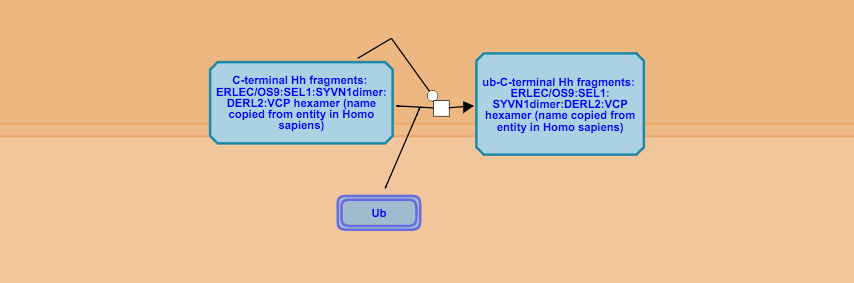
\includegraphics[width=\textwidth]{at_hh}
     \caption[\textit{Arabidopsis thaliana} Hedgehog pathway]{The Reactome Hedgehog signaling pathway in \textit{A. thaliana}. For this pathway, and many others, the Reactome database is very sparse relative to the orthologous pathways in humans, and is therefore not very useful for implementing network algorithms, at this point.}
     \label{fig:at_hh}
     \end{center}
   \end{figure}

   Unfortunately, for many small-scale pathways (such as the Hedgehog pathway), there is not as much pathway data available in pathway databases, since much more research has been done on humans than on any other organism. Fortunately, however, there is enough pathway data available that the overall interactome can be searched and may yield useful outcomes.\par

   \begin{figure}[h]
     \begin{center}
       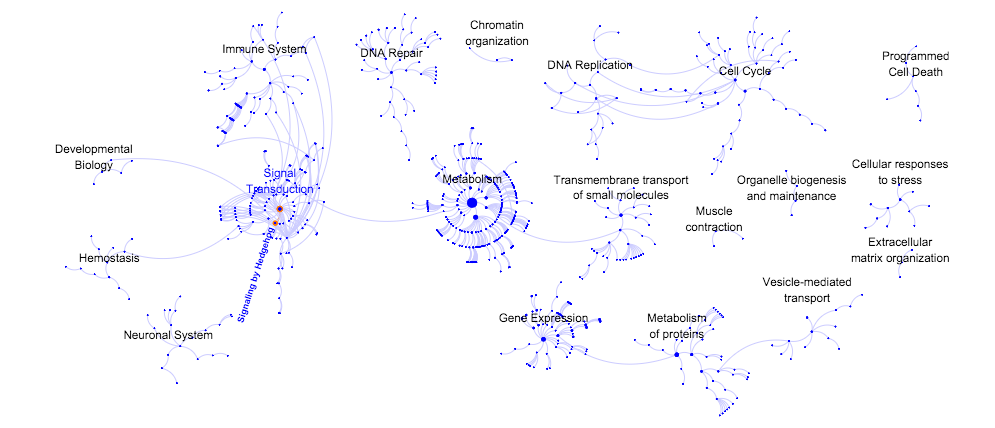
\includegraphics[width=\textwidth]{at_interactome}
     \caption[\textit{Arabidopsis thaliana} interactome]{The entire \textit{A. thaliana}  interactome, as displayed by the Reactome interactive pathway browser. This interactome is similar in size and structure to the human interactome seen in \ref{fig:human_interactome}, though somewhat smaller. This makes it a better candidate for running network algorithms that may not be optimized for a network as large as the human interactome.}
     \label{fig:at_interactome}
     \end{center}
   \end{figure}

   Our ability to look at the entire interactome of species such as \textit{A. thaliana} allows us to investigate some of the global effects of genetic manipulation on signal transduction. This is especially useful in model organisms like \textit{A. thaliana}, since we can actually perform genetic manipulations on them quickly, safely, and ethically, unlike with human beings. Additionally, our ability to breed model organisms in the lab means that we can use specific datasets with large sample sizes. This is very useful compared to human datasets, which are generally based on small sample sizes, since human gene expression data is generally collected from pseudo-random, sparse cases when a person has a degenerate tissue type, such as a tumor, rather than under direct experimental manipulation.\par

   In the future, we wish to optimize our implementation of the weighted subhypernetwork problem, so that it can handle datasets on the scale of an entire interactome, so that we can seek worthy interactions not just in a pathway in which we have \textit{a priori} reasons to search, but rather the whole organismal interactome.

   \subsection{Complexed Hypergraphs}

   We can define sets of two or more nodes as a hypernode, which are members of the power set of $V$.  These can be incorporated into a directed hypergraph to form a \textit{complexed directed hypergraph}.  We define a \textit{complexed directed hypergraph}, $\mathcal{H}$, as the triple $(V,U,E)$ in which $V$ is a finite set of vertices, $U \subseteq 2^V$ is a finite set of hypernodes, and $E \subseteq 2^U \times 2^U$ is a finite set of hyperedges such that, for every $e=(T(e),H(e)) \in E$, $T(e) \cap H(e) = \emptyset$ and $T(e)$, $H(e) \neq \emptyset$. In the future, we hope to extend our ILP formulation to handle hypergraphs with complexes, so that we better model the way in which signals are transduced through cells.\par

   \subsection{Comparison to Standard Graphs}

   To test how well this algorithm is able to construct sub-hypergraphs that are more meaningful than their standard counterparts, we can examine the same implementation on hypergraphs that have been converted to standard graphs. For this conversion, each hyperedge in the original hypergraph will be replaced with a set of directed edges that corresponded to all pairwise tail-to-head connections. By using this comparison, we can determine the extent to which our hypershrub formulation is able to both recapture results that would be found through standard graph analysis, as well as showing us how much new information we were able to gain through our use of a more nuanced way of representing protein-protein interaction networks.



%If you feel it necessary to include an appendix, it goes here.
    \appendix
      \chapter{Examples of Files}

        \paragraph{Construction of LP files.}The constructor \verb|build_lp.py| builds a \texttt{.lp} file that can be optimized by the ILP solver CPLEX. The constructor takes the following files as arguments, as well as a column delimeter (default ``\texttt{;}") and a node delimeter (default ``\texttt{,}").

        Edge file (\texttt{ex-edges.txt}):\\
        \rule{\textwidth}{1pt}
        \verbatiminput{../examples/ex-edges.txt}
        \rule{\textwidth}{1pt}

        \newpage

        Node file (\texttt{ex-nodes.txt}):\\
        \rule{\textwidth}{1pt}
        \verbatiminput{../examples/ex-nodes.txt}
        \rule{\textwidth}{1pt}

        \newpage

        Output file (\texttt{ex.lp}):\\
        \rule{\textwidth}{1pt}
        \begin{lstlisting}
Maximize
 obj: 2.0 Kx + 8.0 Gx + 16.0 Jx + 4.0 Hx + 7.0 Ax + 12.0 Dx + 7.0 Lx + 14.0 Bx + 7.0 Mx + 3.0 Fx + 24.0 Ix + 21.0 Cx + 19.0 Ex - 0.0 Kd - 37.0 Gd - 24.0 Jd - 4.0 Hd - 10.0 Ad - 16.0 Dd - 0.0 Ld - 32.0 Bd - 0.0 Md - 14.0 Fd - 12.0 Id - 1.0 Cd - 98.0 Ed - 31.0 hyperedge8 - 5.0 hyperedge3 - 45.0 hyperedge12 - 33.0 hyperedge6 - 14.0 hyperedge2 - 4.0 hyperedge1 - 12.0 hyperedge10 - 9.0 hyperedge7 - 14.0 hyperedge5 - 57.0 hyperedge4 - 19.0 hyperedge11 - 8.0 hyperedge9
Subject To
 c44_hyperedge8: Jx - 1 hyperedge8 >= 0
 c43_hyperedge8: Ix - 1 hyperedge8 >= 0
 c44_hyperedge3: Cx - 1 hyperedge3 >= 0
 c43_hyperedge3: Fx + Gx - 2 hyperedge3 >= 0
 c44_hyperedge12: Ex - 1 hyperedge12 >= 0
 c43_hyperedge12: Bx - 1 hyperedge12 >= 0
 c44_hyperedge6: Fx + Gx - 2 hyperedge6 >= 0
 c43_hyperedge6: Ix - 1 hyperedge6 >= 0
 c44_hyperedge2: Bx - 1 hyperedge2 >= 0
 c43_hyperedge2: Fx - 1 hyperedge2 >= 0
 c44_hyperedge1: Ax - 1 hyperedge1 >= 0
 c43_hyperedge1: Dx + Bx - 2 hyperedge1 >= 0
 c44_hyperedge10: Ix - 1 hyperedge10 >= 0
 c43_hyperedge10: Lx + Mx - 2 hyperedge10 >= 0
 c44_hyperedge7: Ix - 1 hyperedge7 >= 0
 c43_hyperedge7: Jx - 1 hyperedge7 >= 0
 c44_hyperedge5: Ex - 1 hyperedge5 >= 0
 c43_hyperedge5: Hx + Lx - 2 hyperedge5 >= 0
 c44_hyperedge4: Dx + Ex - 2 hyperedge4 >= 0
 c43_hyperedge4: Hx + Kx - 2 hyperedge4 >= 0
 c44_hyperedge11: Lx - 1 hyperedge11 >= 0
 c43_hyperedge11: Hx + Kx - 2 hyperedge11 >= 0
 c44_hyperedge9: Hx - 1 hyperedge9 >= 0
 c43_hyperedge9: Lx - 1 hyperedge9 >= 0
 c45_A: Ad - Ax <= 0
 c45_B: Bd - Bx <= 0
 c45_C: Cd - Cx <= 0
 c45_D: Dd - Dx <= 0
 c45_E: Ed - Ex <= 0
 c45_F: Fd - Fx <= 0
 c45_G: Gd - Gx <= 0
 c45_H: Hd - Hx <= 0
 c45_I: Id - Ix <= 0
 c45_J: Jd - Jx <= 0
 c45_K: Kd - Kx <= 0
 c45_L: Ld - Lx <= 0
 c45_M: Md - Mx <= 0
 c46_K: Kd - Kx + hyperedge11 + hyperedge4 >= 0
 c46_G: Gd - Gx + hyperedge3 >= 0
 c46_J: Jd - Jx + hyperedge7 >= 0
 c46_H: Hd - Hx + hyperedge5 + hyperedge11 + hyperedge4 >= 0
 c46_A: Ad - Ax >= 0
 c46_D: Dd - Dx + hyperedge1 >= 0
 c46_L: Ld - Lx + hyperedge5 + hyperedge10 + hyperedge9 >= 0
 c46_B: Bd - Bx + hyperedge1 + hyperedge12 >= 0
 c46_M: Md - Mx + hyperedge10 >= 0
 c46_F: Fd - Fx + hyperedge2 + hyperedge3 >= 0
 c46_I: Id - Ix + hyperedge6 + hyperedge8 >= 0
 c46_C: Cd - Cx >= 0
 c46_E: Ed - Ex >= 0
Bounds
 Kx = 1
 Kd = 0
 Lx = 1
 Ld = 0
 Mx = 1
 Md = 0
Binary
 Ax
 Bx
 Cx
 Dx
 Ex
 Fx
 Gx
 Hx
 Ix
 Jx
 Kx
 Lx
 Mx
 Ad
 Bd
 Cd
 Dd
 Ed
 Fd
 Gd
 Hd
 Id
 Jd
 Kd
 Ld
 Md
 hyperedge1
 hyperedge10
 hyperedge11
 hyperedge12
 hyperedge2
 hyperedge3
 hyperedge4
 hyperedge5
 hyperedge6
 hyperedge7
 hyperedge8
 hyperedge9
End

        \end{lstlisting}
        \rule{\textwidth}{1pt}

      \chapter{Version Information}

      This appendix will be concerned with which versions of various softwares were used in the making of this thesis.

      \begin{itemize}
        \item{All code used in this thesis was written in Python3.4 except the program used to parse Reactome, which was a Java file.}
        \item{Linear program files were analyzed using CPLEX Interactive Optimizer 12.6.2.0
  with Simplex.}
        \item{Programs were analyzed on a machine running Debian GNU/Linux 8.4 (``jessie").}
        \item{Statistics about differential expression were calculated with:}
        \begin{itemize}
          \item{R version 3.2.3}
          \item{Biobase 2.30.0}
          \item{GEOquery 2.36.0}
          \item{limma 3.26.8}
        \end{itemize}
        \item{Hypergraphs were constructed from Reactome version 55.}
      \end{itemize}


%This is where endnotes are supposed to go, if you have them.
%I have no idea how endnotes work with LaTeX.

  \backmatter % backmatter makes the index and bibliography appear properly in the t.o.c...

% if you're using bibtex, the next line forces every entry in the bibtex file to be included
% in your bibliography, regardless of whether or not you've cited it in the thesis.
    \nocite{*}

% Rename my bibliography to be called "Works Cited" and not "References" or ``Bibliography''
% \renewcommand{\bibname}{Works Cited}

%    \bibliographystyle{bsts/mla-good} % there are a variety of styles available;
%  \bibliographystyle{plainnat}
% replace ``plainnat'' with the style of choice. You can refer to files in the bsts or APA
% subfolder, e.g.
 \bibliographystyle{APA/apa-good} % or
 \bibliography{thesis}
 % Comment the above two lines and uncomment the next line to use biblatex-chicago.
 %\printbibliography[heading=bibintoc]

% Finally, an index would go here... but it is also optional.
\end{document}
